% !TeX program = xelatex
\documentclass[UTF8,zihao=-4]{oucart}

\usepackage{amssymb,bm}
\usepackage{epstopdf}
\usepackage{tabularx,array,float}
\usepackage{hyperref}
\usepackage{xcolor}
\usepackage{enumitem}
\usepackage{url}
\usepackage{gbt7714}
\usepackage{makecell}
\usepackage{xurl}
\usepackage{indentfirst}
\usepackage{subcaption}

\hypersetup{hidelinks}
\setlength{\parindent}{2em}
\setlength{\emergencystretch}{3em}
\graphicspath{{figures/}{assets/}}
\captionsetup{font=small,labelfont=bf}

\title{流体模拟自动化平台}
\entitle{Fluid Simulation Automation Platform}
\author{李伯辉}
\studentid{22020007040}
\advisor{甘言海}
\department{信息科学与工程学部}{网络空间安全}
\grade{2022}

\cnabstractkeywords{
偏微分方程求解是科学计算、工程仿真与智能建模中的基础问题。针对毕业设计场景中常见的训练脚本分散、结果格式不统一、模型对比不直观以及展示链路不完整等问题，本文设计并实现了一套流体模拟自动化平台。当前平台以二维热方程作为验证案例，对原始物理信息神经网络求解模块和 Fourier Neural Operator 对照结果进行统一整理与展示；在平台结构上，则预留了向更一般流体方程扩展的接口与结果组织方式。

本文所称“自动化”并非指现场重新训练，而是指结果读取自动化、参数匹配自动化、播放展示自动化以及模型对比自动化四个层面。系统保留原始 PINN 求解模块的核心算法结构，仅在参数整理、结果标准化导出和展示适配层进行非侵入式封装。后端采用 FastAPI 构建统一结果访问接口，前端采用 Vue 3 与 ECharts 实现热力图回放、时间轴联动、误差曲线展示和参数化结果播放。与早期在线求解方案不同，当前平台不再触发新的训练任务，而是通过读取已完成的 PINN 预计算结果集，实现“用户填写参数，系统匹配对应结果并播放”的展示机制。

在实验部分，平台统一纳入 PINN 与 FNO 在二维热方程任务上的正式结果。结果表明，PINN 在 \texttt{epoch\_108000} 时的整体 MSE 为 $1.039\times10^{-8}$，整体 RMSE 为 $1.020\times10^{-4}$；FNO 在 \texttt{epoch\_108000} 时的整体 MSE 为 $1.194\times10^{-7}$，整体 RMSE 为 $3.456\times10^{-4}$。在统一方程、统一网格、统一真值和统一评价指标下，PINN 的预测精度高于 FNO，且误差传播更为平缓。与此同时，平台整理了 \texttt{preset\_base}、\texttt{preset\_low\_nu}、\texttt{preset\_small\_dt} 和 \texttt{preset\_high\_nu} 四组真实 PINN 预计算结果，为参数化播放和后续扩展分析提供了数据基础。

本文的主要工作包括：构建统一的结果组织规范；实现原始 PINN 模块的非侵入式平台接入；完成 PINN 与 FNO 在统一热方程任务下的同平台对比分析；实现参数填写后自动映射预计算结果并播放的前端展示机制。本文工作满足了本科毕业设计对系统设计开发的要求，也为论文的学术分析部分提供了真实实验依据。
}{
流体模拟自动化平台；热方程；物理信息神经网络；傅里叶神经算子；可视化系统
}
\enabstractkeywords{
Solving partial differential equations is a fundamental task in scientific computing, engineering simulation, and intelligent modeling. To address fragmented training scripts, inconsistent result formats, inconvenient model comparison, and incomplete presentation pipelines in undergraduate projects, this thesis designs and implements a fluid simulation automation platform. The current validated case is the two-dimensional heat equation, while the platform architecture remains extensible to more general fluid-equation tasks.

In this thesis, “automation” specifically refers to result reading, parameter matching, playback display, and model comparison. The system preserves the core algorithmic structure of the original PINN solver and only performs non-intrusive wrapping at the parameter organization, result-standardization, and presentation-adaptation layers. FastAPI is adopted to provide unified result-access interfaces, while Vue 3 and ECharts are used to realize heatmap playback, timeline interaction, metric visualization, and parameter-driven result replay. Instead of launching new training tasks online, the current platform matches user-input parameters to precomputed PINN result sets and plays the corresponding data directly.

For experiments, the platform integrates the formal PINN and FNO results under the same heat-equation task. At \texttt{epoch\_108000}, the PINN model achieves an overall MSE of $1.039\times10^{-8}$ and an overall RMSE of $1.020\times10^{-4}$, while the FNO model achieves an overall MSE of $1.194\times10^{-7}$ and an overall RMSE of $3.456\times10^{-4}$. Under unified equation settings, grid resolution, analytical ground truth, and evaluation metrics, PINN provides higher accuracy and more stable error propagation for the current task. In addition, four real PINN preset result groups are organized to support parameterized playback and supplementary analysis.
}{
fluid simulation automation platform; heat equation; physics-informed neural network; Fourier neural operator; visualization system
}

\newcommand{\placeholderfigure}[2]{
  \begin{figure}[H]
    \centering
    \fbox{
      \parbox[c][0.26\textheight][c]{0.88\textwidth}{
        \centering
        \zihao{-4} #1
      }
    }
    \caption{#2}
  \end{figure}
}

\begin{document}

\makecover
\makesignature
\makeabstract

\thispagestyle{tableofcontents}
\tableofcontents
\newpage

\pagenumbering{arabic}
\setcounter{page}{1}

\section{绪论}

\subsection{研究背景与意义}

偏微分方程广泛存在于热传导、扩散、流体流动、电磁传播、结构振动和图像处理等问题中，是连接数学建模与工程计算的重要桥梁。传统科学计算领域通常采用有限差分、有限体积、有限元以及谱方法等数值离散框架，对控制方程进行空间与时间上的近似求解\cite{crank1947,evans2010}。这些方法理论基础成熟、数值稳定性研究充分，在热方程、Poisson 方程以及 Navier--Stokes 方程等典型问题上已经形成了完整的方法体系。然而，当问题规模增大、参数空间增广、边界条件复杂或需要频繁重复求解时，传统数值方法在建模效率、结果管理以及跨任务复用方面仍然面临较高成本。

近年来，深度学习在函数逼近和高维表达方面显示出较强能力，使其逐步进入偏微分方程求解研究领域。尤其是在数据获取困难、方程结构已知但解析求解复杂、或者需要快速构建代理模型的场景中，深度学习为传统数值方法提供了新的补充思路。以 PINN 为代表的物理信息神经网络方法，通过把方程残差、边界条件和初始条件嵌入损失函数，把神经网络训练与物理约束结合起来，在小样本或无显式标签样本条件下仍然能够获得具有物理一致性的近似解\cite{raissi2019,karniadakis2021}。以 FNO 为代表的神经算子方法，则进一步尝试学习“函数到函数”的映射关系，在参数化偏微分方程、多样本算子逼近和跨实例泛化方面表现出新的潜力\cite{li2021fno,kovachki2023}。

从工程展示角度看，毕业设计中的一个突出问题并不只是“模型能否训练成功”，而是“能否形成稳定、完整、可演示、可复现的系统链路”。实际项目开发中，训练脚本、结果文件、误差统计、可视化页面和论文图表往往分散在不同目录与不同脚本中，导致以下几个问题：其一，训练所得结果难以统一管理，模型间对比依赖人工整理；其二，前端展示往往只能静态截图，缺少时间步联动和误差曲线联动；其三，答辩展示场景强调系统稳定性，不适合现场长时间训练等待；其四，论文内容容易在“代码复现”与“系统开发”之间失去平衡，难以同时体现工程性和学术性。

因此，本课题的意义不在于重新提出一套全新的基础求解理论，而在于围绕真实的 PINN 求解模块和 FNO 对照结果，构建一套适合毕业设计场景的流体模拟自动化平台。一方面，该平台能够完成结果标准化、接口组织和前端联动展示，提高项目的工程完整度；另一方面，通过在同一平台下纳入 PINN 与 FNO 的热方程结果，平台又能够为论文中的模型对比分析提供统一的数据载体和实验支撑。这里“自动化”的含义主要体现在四个方面：其一，系统能够自动读取并识别统一目录下的结果集；其二，能够依据用户填写参数自动匹配对应预计算结果；其三，能够自动完成热力图、时间轴和误差曲线的联动播放；其四，能够自动组织 PINN、FNO、Ground Truth 和差异图的同屏比较。对本科毕业设计而言，这种“系统平台为主、算法分析为辅，但两者互相支撑”的路线更能体现综合能力。

本文将二维热方程作为统一验证对象，其原因主要有三点。首先，热方程具有明确的物理背景和较成熟的数值分析理论；其次，其解析解已知，便于以严格真值为基准评估模型结果；再次，热方程的时间演化特征直观，适合通过热力图、差异图和误差曲线进行网页展示。这使得热方程既能作为平台功能验证对象，也能作为 PINN 与 FNO 对比分析的实验载体。需要说明的是，论文当前所有正式实验与页面展示都围绕二维热方程展开，它承担的是“平台验证案例”的角色；而平台在结果目录组织、接口层设计和前端展示层设计上，并未把方程类型永久限定为热方程，因此后续可继续扩展至 Poisson 方程、Burgers 方程以及更一般的流体方程任务。

结合以上背景，本文所构建的平台不仅面向结果播放和演示，更面向“结果如何被统一组织、如何被参数映射调用、如何支持对比分析、如何服务论文写作与答辩展示”这一完整问题。其研究意义体现在三个层面：一是为本科毕业设计形成一条从训练结果到平台展示再到论文图表的完整工作流；二是为 PINN 与 FNO 在统一任务下的同平台比较提供可靠基础；三是为今后扩展到更多偏微分方程和更多离线结果集提供可复用框架。

\subsection{国内外研究现状}

\subsubsection{传统偏微分方程数值求解研究现状}

传统偏微分方程求解长期依赖有限差分、有限元、有限体积以及谱方法等数值框架。Crank 与 Nicolson 提出的经典时间离散思想在热传导方程求解中具有代表性\cite{crank1947}，而 Evans 的偏微分方程教材则系统总结了控制方程、边界条件、适定性和数值分析等基本理论\cite{evans2010}。这些传统方法的优势在于数学基础稳固、误差分析清晰、结果可靠性高，因此在工业仿真和科学计算中仍然占据主导地位。

但与此同时，传统数值方法通常是“面向单个问题的精确计算方法”，而不是“面向结果快速复用的学习型方法”。在同类方程反复求解、参数变化频繁或需要快速展示大量结果的场景下，传统数值求解往往面临重复计算成本高、结果格式不统一以及工程集成难度大的问题。对于本科毕业设计平台开发而言，单纯依赖传统数值解法虽然能保证结果精度，但难以直接体现模型比较、结果复用和交互展示等现代计算平台特征。因此，基于深度学习的 PDE 求解方法逐渐受到关注。

\subsubsection{物理信息神经网络研究现状}

PINN 是近年偏微分方程学习求解领域最具代表性的方法之一。Raissi、Perdikaris 和 Karniadakis 在 2019 年发表于《Journal of Computational Physics》的论文中正式提出了 Physics-informed Neural Networks 的统一框架\cite{raissi2019}。该工作指出，可以通过自动微分获得网络输出对时空坐标的导数，再将偏微分方程残差与初边值约束嵌入损失函数，从而把监督学习、方程约束和系统识别统一到同一训练过程之中。这篇论文同时给出了连续时间模型与离散时间模型两条路线，并通过 Burgers 方程、Schrödinger 方程、Allen--Cahn 方程以及 Navier--Stokes 方程等案例验证了框架的有效性。

随后，PINN 研究迅速发展。Karniadakis 等从物理信息机器学习角度对这一方向进行了系统总结，指出 PINN 的优势在于可融合先验物理知识、适应小样本问题，并有望改善传统纯数据驱动模型对数据规模的依赖\cite{karniadakis2021}。Cuomo 等进一步从科学机器学习视角综述了 PINN 在算法结构、损失构造、优化策略和工程应用方面的发展脉络，强调其在复杂多物理场建模中的潜力，同时也指出了训练刚性、梯度失衡、误差传播和泛化能力不足等问题\cite{cuomo2022}。Cai 等则面向流体力学任务对 PINN 的研究进展进行了回顾，说明 PINN 在稳态/非稳态流动重建、参数反演和边界估计方面具有较强吸引力，但在高雷诺数流动和强非线性问题中仍存在训练困难\cite{cai2021fluid}。

在中文研究中，查文舒等对基于神经网络的偏微分方程求解方法进行了综述，系统梳理了数据驱动、物理约束以及物理驱动三类思路的区别和联系，为国内研究者理解 PINN 方法提供了较为清晰的框架\cite{zha2022review}。李野等围绕物理信息神经网络的理论基础、训练机制和应用场景，分析了该方法在方程残差建模、自动微分、样本需求和物理一致性方面的特点\cite{liye2022pinnreview}。陈煜谦的学位论文则进一步把 PINN 放到更广泛的“深度学习求解偏微分方程”背景下讨论，为本科阶段开展此类研究提供了较好的中文参考\cite{chen2024deeppde}。

总体来看，国内外关于 PINN 的研究已从“方法提出”进入“结构改进、训练策略优化与应用拓展”阶段。其理论价值体现在把物理先验显式引入神经网络训练；工程价值则体现在对复杂 PDE 任务提供了新的代理求解路径。本文平台所使用的原始 PINN 求解模块虽非标准教材式最简 PINN，但其核心仍属于“物理约束参与训练、网络输出遵循热方程演化规律”的物理信息求解范畴，因此在论文中以 PINN 作为主模型分析对象是合理的。

\subsubsection{神经算子与 FNO 研究现状}

与 PINN 直接学习方程解不同，神经算子方法更强调学习“函数到函数”的映射关系。DeepONet 从算子泛函逼近的角度，证明了神经网络学习非线性算子的可行性，为参数化偏微分方程和多实例任务求解提供了理论基础\cite{lu2021deeponet}。在此基础上，Li 等提出了 Fourier Neural Operator，通过在频域中学习卷积核参数，实现了对参数化 PDE 解算子的高效逼近\cite{li2021fno}。这一方法在速度、批量推理和跨实例泛化方面表现出较大优势，因此迅速成为神经算子研究的代表模型。

Kovachki 等随后在《Journal of Machine Learning Research》发表综述性工作，对 Neural Operator 的理论框架、逼近能力、函数空间映射性质和应用方向进行了系统总结\cite{kovachki2023}。相关研究表明，神经算子方法特别适合处理多样本、多参数、可重复调用的 PDE 代理建模问题，这与传统“单样本精解”的数值计算路线有所不同。对于需要大量重复求解、批量预测和快速推理的工程场景，FNO 及其后续变体具有较强吸引力。

中文研究中，刘泳成围绕融合数学物理知识的神经网络算子方法展开了系统研究，对神经算子在物理场映射、算子学习和多任务建模中的潜力进行了较深入讨论\cite{liu2026operator}。陈煜谦的研究同样把 FNO、DeepONet 等方法纳入深度学习求解偏微分方程的整体框架中，为本文开展 PINN 与 FNO 的对比分析提供了中文研究支撑\cite{chen2024deeppde}。

然而，从目前研究现状看，FNO 的优势更多体现在大规模样本学习和算子级泛化，而不是在每一个特定小规模任务中都优于 PINN。在热方程这样解析结构较明确、任务规模有限、并且训练链路高度受物理约束的问题上，PINN 与 FNO 的表现并不存在先验上谁绝对更优的问题，这也正是本文开展同平台对比的实际价值所在。通过统一的结果组织与统一的可视化展示，本文能够更直接地回答“在当前热方程任务上，原始 PINN 与离线 FNO 对照结果各有什么特点”。

\subsubsection{平台化展示与系统集成研究现状}

相较于算法本身，面向毕业设计和教学演示的“结果组织 + 接口服务 + 网页展示”平台研究明显较少。现有相关工作多集中于科学计算结果可视化系统、Web 数据展示平台或仿真辅助教学系统，但往往缺少对神经网络 PDE 结果的统一结构设计。尤其是在一个平台内同时支持参数映射播放、时间帧联动、模型差异热力图和误差曲线展示的工作并不常见。

从工程实现角度看，FastAPI 在轻量级接口服务、异步结果访问和 JSON 数据组织方面具有较好实用性\cite{fastapi_docs}；Vue 3 适合管理复杂前端状态和双向交互逻辑\cite{vue_docs}；ECharts 则适合实现热力图、曲线图和多图联动展示\cite{echarts_docs}。这些现代 Web 技术为构建偏微分方程结果展示平台提供了较好的工程基础。

但如果缺少统一结果标准，上层前端往往无法直接复用不同模型的输出。本文的工作重点之一正是在此处：以统一目录结构、统一元数据文件和统一逐帧场数据接口，把原始 PINN 结果、FNO 对照结果和 PINN 参数化预计算结果整理到同一平台中。与单纯实现一个前端页面相比，这种“离线训练结果标准化 + 同平台调用 + 可视化回放”的整合方式，更符合毕业设计“系统开发 + 实验分析”的双重要求。

\subsection{研究内容}

本文围绕流体模拟自动化平台展开，主要研究内容包括：
\begin{enumerate}[label=\arabic*)]
  \item 以二维热方程为统一验证对象，整理并接入原始 PINN 求解模块的正式训练结果；
  \item 将 FNO 对照结果纳入同一目录规范和同一接口规范，构建统一结果访问机制；
  \item 设计结果标准化导出结构，统一组织热力图、真值场、差异场、元数据和误差指标；
  \item 设计基于 FastAPI 的结果接口与基于 Vue 3 的可视化前端，形成完整展示链路；
  \item 实现 PINN 参数化结果回放与 PINN/FNO 对比分析的双模块页面结构；
  \item 基于正式实验结果，完成 PINN 与 FNO 在统一热方程任务下的误差对比分析。
\end{enumerate}

\subsection{本文主要工作与贡献}

本文的主要工作与贡献可概括为以下几个方面：
\begin{enumerate}[label=\arabic*)]
  \item 在不改动原始 PINN 求解核心思路的前提下，实现了面向展示平台的非侵入式系统接入；
  \item 构建了统一的结果组织与接口访问规范，使 PINN、FNO 与解析真值能够在同一平台下进行对比展示；
  \item 采用“参数填写后匹配预计算结果集”的方式替代在线求解，有效提高了系统演示稳定性和答辩适用性；
  \item 结合 PINN 与 FNO 的正式实验结果，形成了具有学术分析价值的同平台比较流程。
\end{enumerate}

\section{相关理论与关键技术}

\subsection{二维热方程模型}

本文采用的控制方程为
\begin{equation}
\frac{\partial u}{\partial t}=\nu\left(\frac{\partial^2u}{\partial x^2}+\frac{\partial^2u}{\partial y^2}\right),
\end{equation}
其中，$u(x,y,t)$ 表示温度场，$\nu$ 为扩散系数。定义区域为 $\Omega=[0,1]\times[0,1]$，初始条件为
\begin{equation}
u(x,y,0)=\sin(\pi x)\sin(\pi y),
\end{equation}
边界条件为零 Dirichlet 边界。对应解析解为
\begin{equation}
u(x,y,t)=\exp(-2\pi^2\nu t)\sin(\pi x)\sin(\pi y).
\end{equation}
由于解析解可直接获得，本文能够以严格真值为基准，对不同模型结果进行误差分析。

\subsection{原始 PINN 求解模块原理}

本文所用主求解链路来源于既有原始 PINN 求解模块。其核心思想不是简单地把方程解当作纯数据拟合对象，而是结合解析真值生成、时间推进、物理残差约束和神经网络修正机制完成热方程演化学习。该模块在训练时，首先生成热方程在固定网格上的短时真值序列，再构造相邻时刻的输入输出对；随后通过数据驱动前向传播模块预测下一时刻温度场，并以物理残差项作为主要损失，约束预测结果满足热方程演化规律。

从标准 PINN 角度看，若以神经网络 $u_\theta(x,y,t)$ 近似热方程解，则热方程残差可写为
\begin{equation}
r_\theta(x,y,t)=\frac{\partial u_\theta}{\partial t}-\nu\left(\frac{\partial^2 u_\theta}{\partial x^2}+\frac{\partial^2 u_\theta}{\partial y^2}\right).
\end{equation}
标准 PINN 的总损失函数通常写为
\begin{equation}
\mathcal{L}=\lambda_f\mathcal{L}_f+\lambda_i\mathcal{L}_i+\lambda_b\mathcal{L}_b,
\end{equation}
其中
\begin{equation}
\mathcal{L}_f=\frac{1}{N_f}\sum_{n=1}^{N_f}\left|r_\theta(x_n,y_n,t_n)\right|^2,
\end{equation}
\begin{equation}
\mathcal{L}_i=\frac{1}{N_i}\sum_{n=1}^{N_i}\left|u_\theta(x_n,y_n,0)-u_0(x_n,y_n)\right|^2,
\end{equation}
\begin{equation}
\mathcal{L}_b=\frac{1}{N_b}\sum_{n=1}^{N_b}\left|u_\theta(x_n,y_n,t_n)-g(x_n,y_n,t_n)\right|^2.
\end{equation}
这里 $\mathcal{L}_f$ 对应方程残差损失，$\mathcal{L}_i$ 对应初始条件损失，$\mathcal{L}_b$ 对应边界条件损失，$\lambda_f,\lambda_i,\lambda_b$ 为各项权重。在本文平台所接入的原始求解模块中，训练实现并非完全照搬上述最简形式，而是采用“物理约束为主、网络修正演化为辅”的具体工程实现；但其理论出发点与标准 PINN 一致，即通过物理残差约束保证网络预测满足热方程演化规律。

从代码结构上看，该求解模块使用固定网格 $101\times101$、时间步长 $dt=10^{-5}$、扩散系数 $\nu=1.0$，并以内置解析解作为训练与测试基准。网络内部结合卷积与 Transformer 修正结构，使得模型能够学习由当前温度场到后续温度场的演化映射。尽管该实现不是标准教科书式最简 PINN 结构，但其本质仍属于“以物理约束为主、以神经网络为近似器”的物理信息求解框架，符合 PINN 方法的基本思想\cite{raissi2019,karniadakis2021}。

\subsection{FNO 对照模型原理}

FNO 的核心并非通过自动微分构造方程残差，而是学习函数到函数的映射。其基本更新形式可表示为
\begin{equation}
v_{l+1}(x)=\sigma\left(Wv_l(x)+\mathcal{F}^{-1}\left(R\cdot \mathcal{F}(v_l)\right)(x)\right),
\end{equation}
其中 $\mathcal{F}$ 表示傅里叶变换，$R$ 为频域可学习参数，$W$ 为局部线性映射。通过在频域中截取主要模态并学习其变换系数，FNO 能够高效逼近参数化偏微分方程的解算子\cite{li2021fno,kovachki2023}。

在本文中，FNO 不承担在线求解角色，而是作为离线对照模型接入平台。平台对其输出进行统一整理后，用于与 PINN 进行同任务、同时间步、同网格规模下的可视化比较与误差分析。

\subsection{平台关键技术}

平台后端采用 FastAPI 构建统一结果访问接口，用于读取结果目录、元数据、逐帧场数据和误差指标\cite{fastapi_docs}。前端采用 Vue 3 管理页面状态、参数映射和播放逻辑\cite{vue_docs}，并使用 ECharts 实现热力图、误差曲线和多图联动展示\cite{echarts_docs}。通过这些技术组合，平台形成了“结果标准化导出—统一接口访问—网页交互播放—图表联动分析”的完整链路。

\section{系统需求分析与总体设计}

\subsection{功能需求分析}

平台需要满足以下核心功能：
\begin{enumerate}[label=\arabic*)]
  \item 支持浏览 PINN 与 FNO 的正式结果集；
  \item 支持热力图逐帧播放与时间轴联动；
  \item 支持填写 PINN 参数并映射到对应预计算结果集；
  \item 支持同一页面下的 PINN/FNO 对比分析；
  \item 支持展示误差曲线、差异热力图和元数据摘要。
\end{enumerate}

\subsection{非功能需求分析}

\begin{enumerate}[label=\arabic*)]
  \item 非侵入式：不改动原始 PINN 核心算法逻辑；
  \item 稳定性：答辩场景不依赖现场重新训练；
  \item 一致性：不同模型结果采用统一目录结构与统一接口；
  \item 可复现性：页面展示全部基于已完成训练结果；
  \item 可扩展性：后续可增加更多方程或更多离线结果集。
\end{enumerate}

\subsection{系统总体架构设计}

平台总体采用“结果层—接口层—展示层”三层结构。结果层负责存储 PINN、FNO 与 PINN 预设参数结果；接口层负责读取统一目录下的热力图数组、元数据和误差指标；展示层负责完成参数填写、结果映射、时间播放和模型对比。该结构使平台能够在不改动原始求解主链路的情况下，实现结果管理与演示功能的解耦。

\begin{figure}[H]
  \centering
  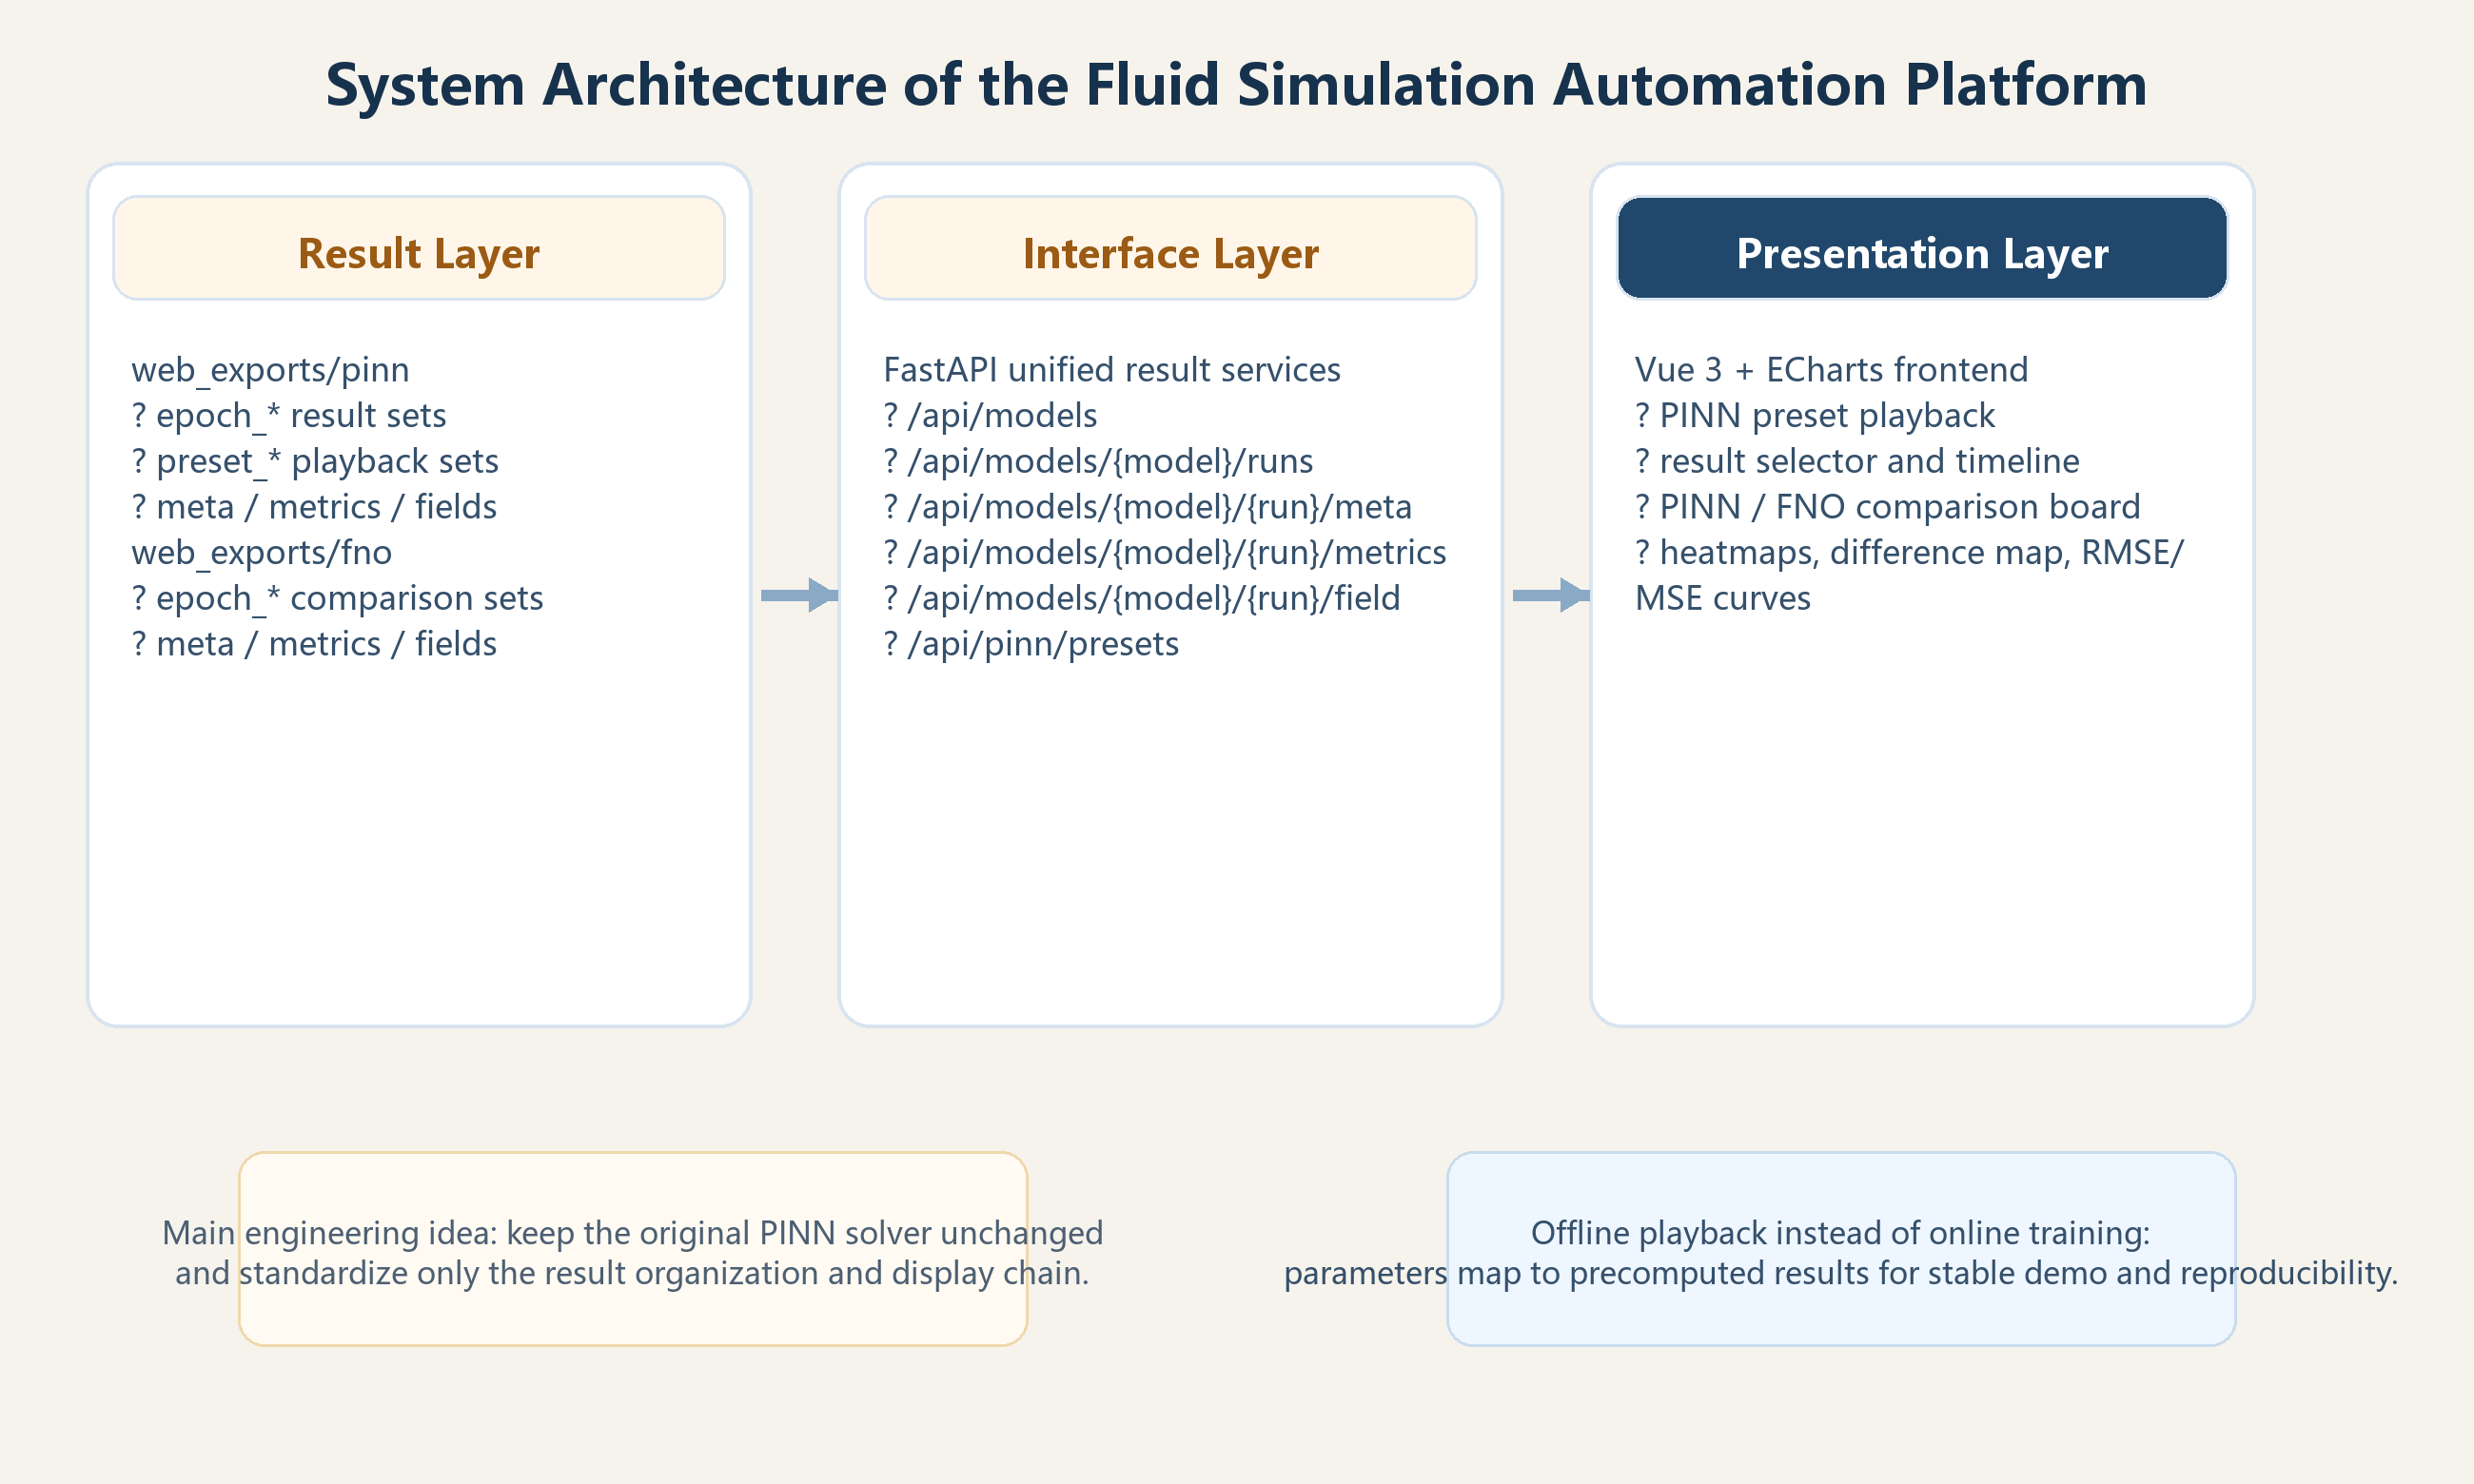
\includegraphics[width=0.9\textwidth]{fig3_1_system_architecture.png}
  \caption{系统总体架构图}
\end{figure}

\subsection{统一结果导出设计}

平台对所有结果采用统一结构组织：
\begin{verbatim}
web_exports/
  pinn/
    epoch_012000/
    epoch_060000/
    epoch_108000/
    preset_base/
    preset_low_nu/
    preset_small_dt/
    preset_high_nu/
  fno/
    epoch_012000/
    epoch_060000/
    epoch_108000/
\end{verbatim}

每个结果目录包含预测场、真值场、差异场、元数据文件和误差指标文件，从而保证前端在读取不同模型结果时无需区分其内部训练来源。以单个结果目录为例，其核心文件及含义如表 \ref{tab:exportfiles} 所示。

\begin{table}[H]
  \centering
  \caption{统一结果目录核心文件说明}
  \label{tab:exportfiles}
  \small
  \begin{tabularx}{0.96\textwidth}{>{\ttfamily\raggedright\arraybackslash}p{4.2cm} X}
    \toprule
    文件名 & 作用说明 \\
    \midrule
    meta.json & 记录模型名称、结果来源、网格尺寸、时间步长、短时/长时帧数、参数标签等元信息，用于页面摘要展示和结果识别。 \\
    metrics.json & 记录整体 MSE、整体 RMSE、逐帧 \texttt{frame\_mse}、逐帧 \texttt{frame\_rmse} 等误差指标，用于误差曲线绘制与整体比较。 \\
    prediction\_short.npy & 存储短时演化窗口下的预测温度场序列，数组维度可理解为“时间帧 $\times$ 高度 $\times$ 宽度”。 \\
    gt\_short.npy & 存储短时演化窗口下的解析真值温度场序列，用于与预测结果逐帧比较。 \\
    diff\_short.npy & 存储短时演化窗口下预测结果与真值的逐点差值场。 \\
    prediction\_long.npy / gt\_long.npy / diff\_long.npy & 与短时窗口对应，但用于更长时间推进的回放与误差分析。 \\
    \bottomrule
  \end{tabularx}
\end{table}

其中，\texttt{meta.json} 更偏向“结果身份说明文件”，\texttt{metrics.json} 更偏向“评价指标汇总文件”，而 \texttt{*.npy} 场数据文件则是前端逐帧热力图播放的直接数据来源。通过这种分工，平台能够在不重新理解训练细节的前提下，完成不同结果集的统一读取与统一展示。

\subsection{参数回放与结果映射机制}

与在线求解方式不同，当前平台采取“参数填写后匹配预计算结果”的回放机制。用户在页面中填写方程类型、扩散系数、时间步长、训练轮次和结构参数后，系统依据预先登记的参数组进行一一匹配；若匹配成功，则自动切换到对应结果集并播放其热图与误差结果；若匹配失败，则提示当前参数尚无对应结果。该机制兼顾了交互性和稳定性，是平台设计中的关键取舍。

\begin{figure}[H]
  \centering
  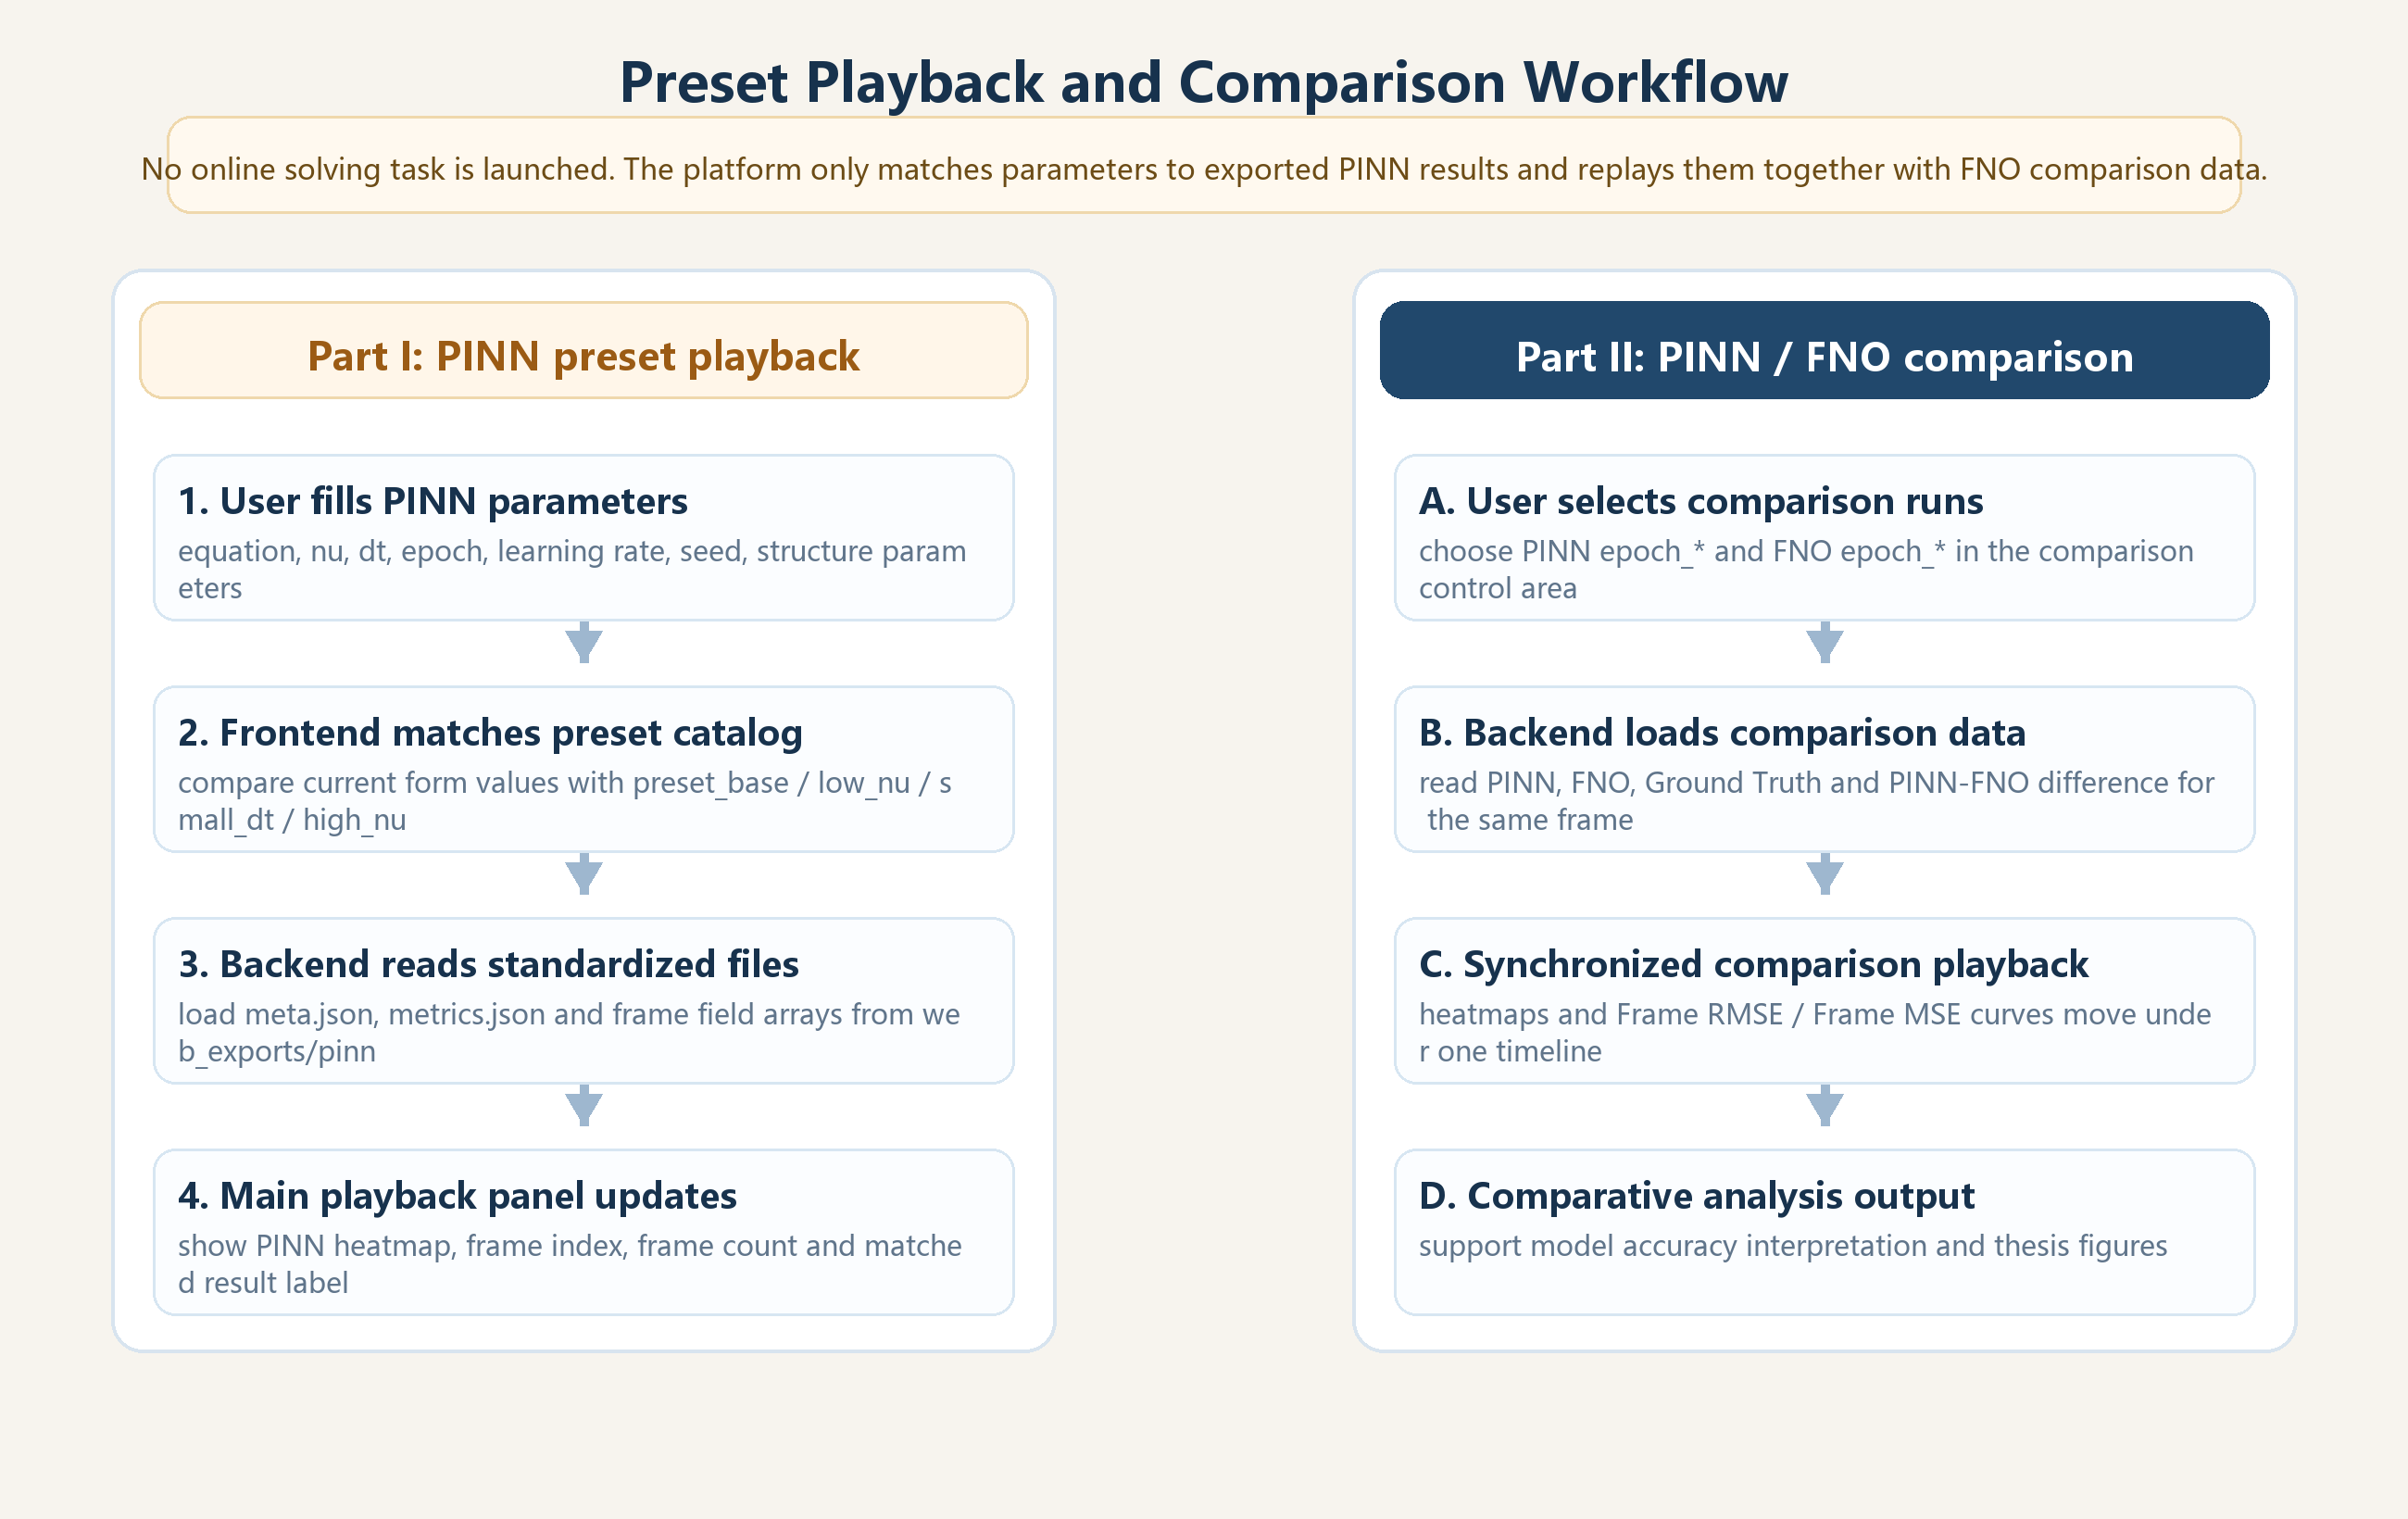
\includegraphics[width=0.9\textwidth]{fig4_1_runtime_workflow.png}
  \caption{参数回放与对比播放流程图}
\end{figure}

\section{平台实现}

\subsection{PINN 模块接入与结果整理}

平台不直接重写原始 PINN 模块，而是围绕其结果导出进行整理。原始模块会在训练过程中周期性保存不同轮次的二维热场预测结果，平台将其转换为统一的 \texttt{web\_exports} 结构，并补充元数据和逐帧误差指标。这一过程实现了“原始求解模块不变，平台层标准化接入”的设计目标。

\subsection{FNO 对照结果接入}

FNO 结果采用离线接入方式，与 PINN 一样整理为统一目录结构。平台在对比分析区同步读取 PINN、FNO 与 Ground Truth 三类结果，并绘制 PINN--FNO 差异图以及误差曲线。由此形成“参数化演示以 PINN 为主、学术性比较以 PINN/FNO 对比为主”的展示格局。

\subsection{后端接口实现}

后端主要接口如表 \ref{tab:api} 所示。
\begin{table}[H]
  \centering
  \caption{后端主要接口说明}
  \label{tab:api}
  \small
  \begin{tabularx}{0.95\textwidth}{>{\ttfamily\raggedright\arraybackslash}p{5.8cm} >{\centering\arraybackslash}p{1.2cm} X}
    \toprule
    接口 & 方法 & 功能 \\
    \midrule
    /api/models & GET & 列出可用模型目录 \\
    /api/models/\{model\}/runs & GET & 列出指定模型下的结果集目录 \\
    /api/models/\{model\}/\{run\}/meta & GET & 返回元数据 \\
    \makecell[l]{/api/models/\{model\}/\{run\}/\\metrics} & GET & 返回整体与逐帧误差 \\
    \makecell[l]{/api/models/\{model\}/\{run\}/\\field} & GET & 返回指定时间帧的二维场数据 \\
    /api/compare/\{epoch\} & GET & 返回 PINN 与 FNO 对比场数据 \\
    /api/pinn/presets & GET & 返回 PINN 预计算参数组 \\
    \bottomrule
  \end{tabularx}
\end{table}

各接口的输入输出可进一步概括为：\texttt{/api/models} 用于返回可用模型名称列表；\texttt{/api/models/\{model\}/runs} 输入模型名，输出对应结果集目录数组；\texttt{/api/models/\{model\}/\{run\}/meta} 输入模型名和结果集名，输出该结果集的网格信息、帧数和参数标签；\texttt{/api/models/\{model\}/\{run\}/metrics} 输出整体误差与逐帧误差数组；\texttt{/api/models/\{model\}/\{run\}/field} 则依据 \texttt{kind} 和时间索引 \texttt{t} 返回单帧二维场数据；\texttt{/api/pinn/presets} 返回前端参数回放所需的预设参数组及其运行标识。

以后端读取单帧场数据为例，其核心处理流程可概括为如下伪代码：
\begin{verbatim}
input: model, run, kind, t
1. 定位 web_exports/model/run 目录
2. 读取 kind 对应的 .npy 场数据文件
3. 检查时间索引 t 是否在合法范围内
4. 取出第 t 帧二维数组
5. 以 JSON 形式返回 field、shape 和 frameIndex
\end{verbatim}
该流程说明后端的主要职责并不是重新计算方程解，而是对统一结果结构进行标准化读取、索引检查和接口封装。

\subsection{前端页面实现}

前端页面被划分为两个相互衔接但职责不同的区域。

\textbf{第一部分：PINN 参数化演示。}  
用户填写参数后，系统不再执行新的训练任务，而是根据参数匹配 \texttt{preset\_*} 结果集，并在主热力图中回放对应 PINN 结果。该区域主要由“结果集与时间轴”和“PINN 参数化演示”两张卡片组成：前者负责时间窗选择、PINN 结果集选择、播放按钮与时间轴控制；后者负责展示预设结果组、参数填写表单以及参数匹配状态。二者共同构成“参数填写—结果映射—热图播放”的主交互流程。

\textbf{第二部分：PINN 与 FNO 对比分析。}  
页面提供独立的对比播放控制，用于同步显示 PINN、FNO、Ground Truth 与差异图，并联动 Frame RMSE 与 Frame MSE 曲线。该部分强调“同任务、同时间轴、同平台”的模型比较能力。界面在视觉上将主演示区与对比分析区上下分层：上层聚焦参数化回放，下层聚焦模型比较与误差分析，使系统展示逻辑更清晰，也更适合毕业答辩场景下的逐步讲解。图 \ref{fig:frontendpinn} 与图 \ref{fig:frontendcompare} 分别展示了这两个区域的页面细节。

\begin{figure}[htbp]
  \centering
  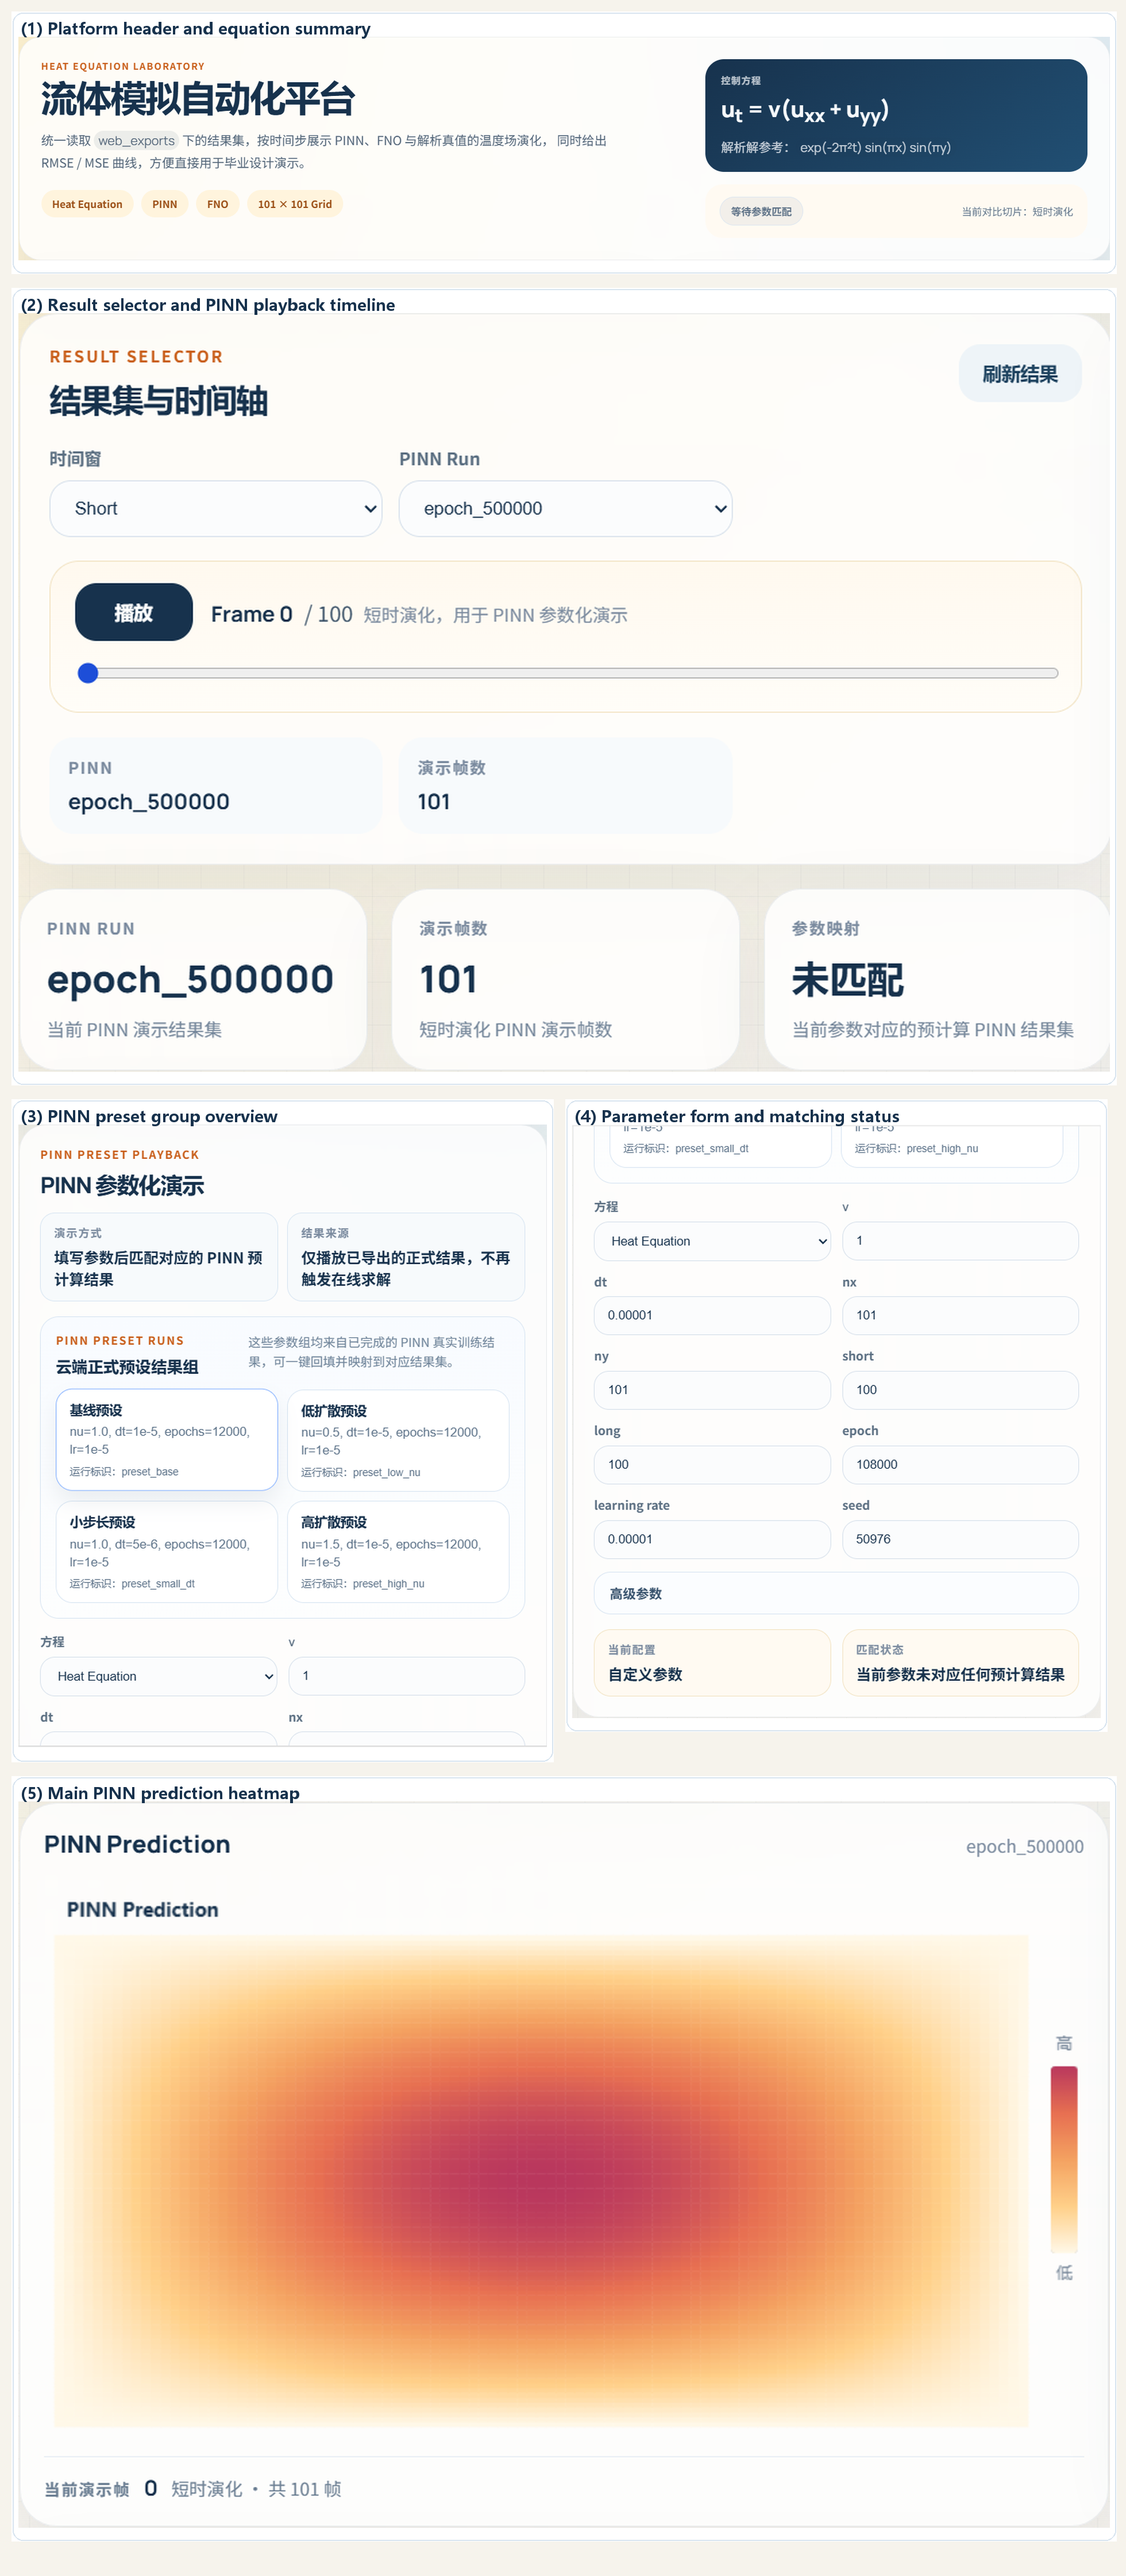
\includegraphics[width=0.94\textwidth]{fig4_2_frontend_pinn_playback.png}
  \caption{PINN 参数化演示模块前端截图}
  \label{fig:frontendpinn}
\end{figure}

\begin{figure}[htbp]
  \centering
  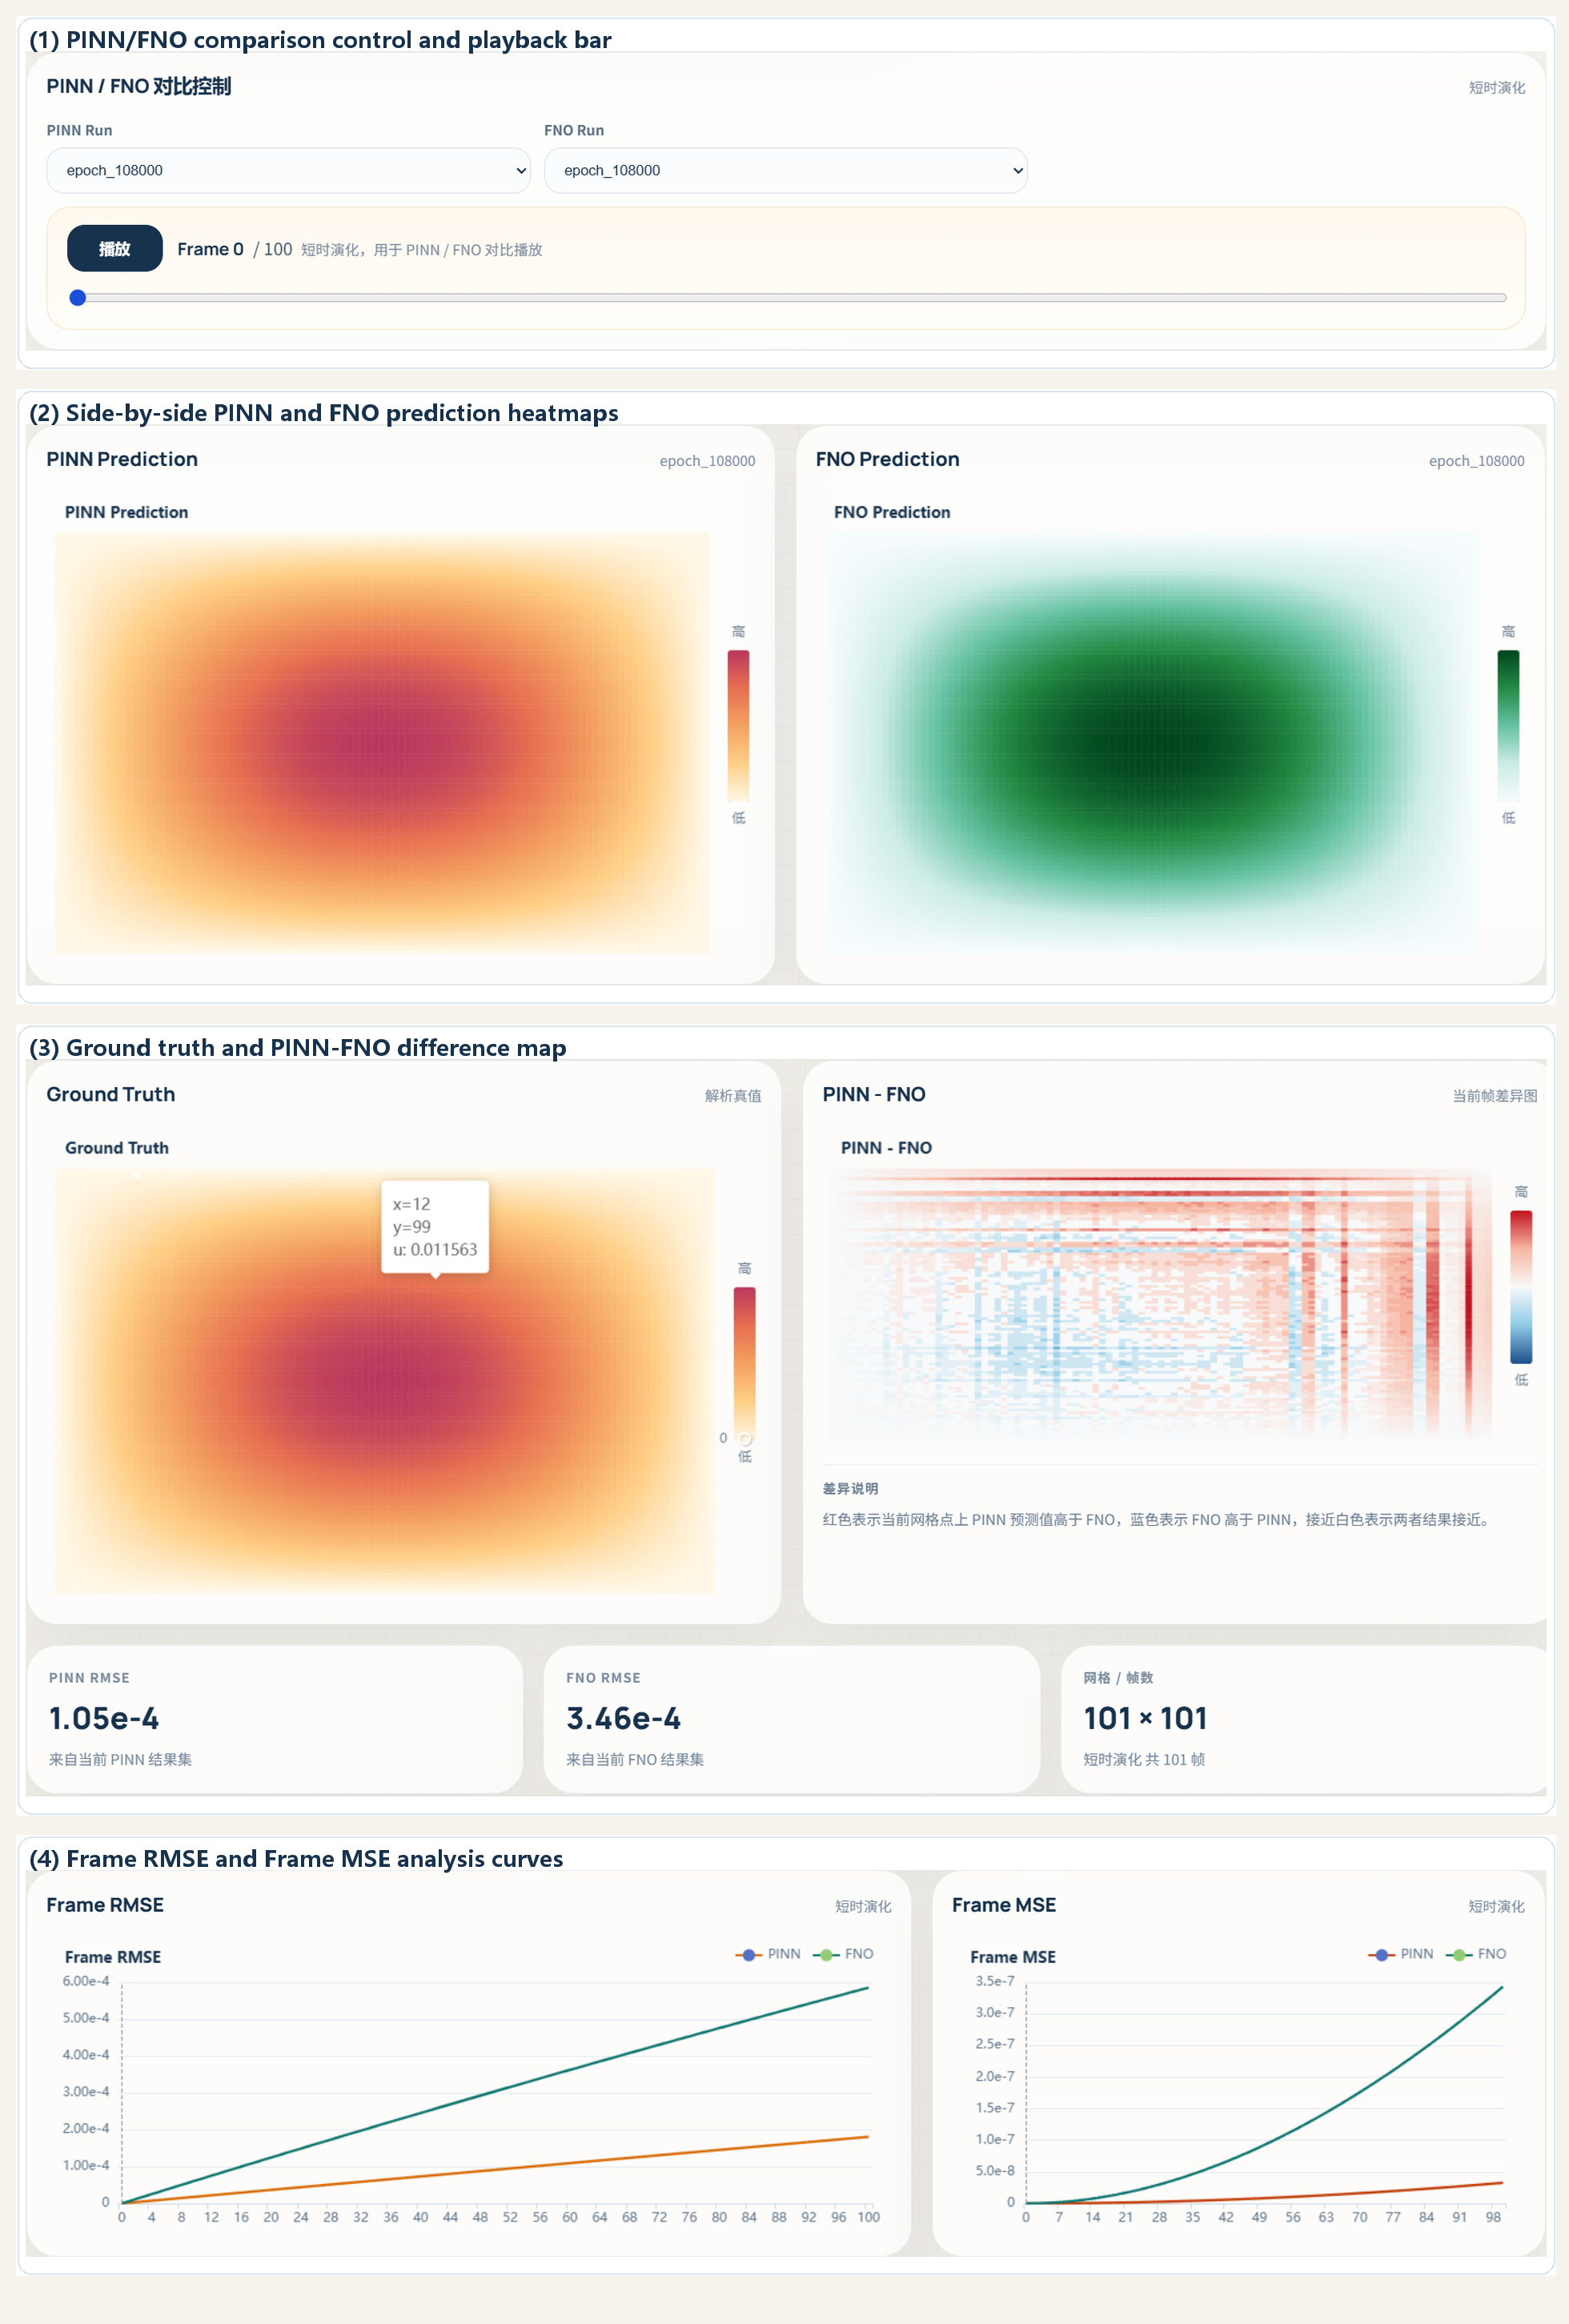
\includegraphics[width=0.94\textwidth]{fig4_3_frontend_compare_module.png}
  \caption{PINN/FNO 对比分析模块前端截图}
  \label{fig:frontendcompare}
\end{figure}

从当前页面结构看，前端展示主要具有以下特点：
\begin{enumerate}[label=\arabic*)]
  \item 头部区域集中展示平台标题、控制方程与解析解摘要，为用户提供统一任务背景；
  \item 左侧上部以时间轴和播放条为核心，突出 PINN 参数化结果的逐帧回放；
  \item 右侧表单区通过参数输入和预设结果组，实现“参数填写后映射到预计算结果”的交互逻辑；
  \item 下部单独设置 PINN/FNO 对比控制区，并联动四张热力图与两张误差曲线，便于从空间分布和整体误差两个层面分析模型差异。
\end{enumerate}

\subsection{参数回放实现机制}

平台当前预置四组正式 PINN 结果集，分别为 \texttt{preset\_base}、\texttt{preset\_low\_nu}、\texttt{preset\_small\_dt} 和 \texttt{preset\_high\_nu}。前端在填写参数后，依据 \texttt{equation}、\texttt{nu}、\texttt{dt}、\texttt{epochs}、\texttt{learning\_rate}、\texttt{seed} 以及结构超参数进行精确匹配；若匹配成功，则自动切换对应结果并更新 PINN 演示热图。其本质是“参数到结果”的映射，而非“参数到在线求解”的计算。

\section{实验设计与结果分析}

\subsection{实验环境与参数配置}

云端训练环境采用 Ubuntu 22.04、Python 3.10.12、NVIDIA GeForce RTX 4090 和 PyTorch 2.5.1+cu121。本地展示环境采用 Windows、FastAPI、Vue 3、Vite 与 ECharts。统一实验网格为 $101\times101$，默认时间步长为 $1\times10^{-5}$。

\begin{table}[H]
  \centering
  \caption{PINN 预设参数组说明}
  \label{tab:preset}
  \begin{tabular}{lllll}
    \toprule
    结果集标识 & $\nu$ & $dt$ & 训练轮次 & short RMSE \\
    \midrule
    preset\_base & $1.0$ & $1\times10^{-5}$ & 12000 & $1.1541\times10^{-4}$ \\
    preset\_low\_nu & $0.5$ & $1\times10^{-5}$ & 12000 & $5.8371\times10^{-5}$ \\
    preset\_small\_dt & $1.0$ & $5\times10^{-6}$ & 12000 & $5.6150\times10^{-5}$ \\
    preset\_high\_nu & $1.5$ & $1\times10^{-5}$ & 12000 & $1.6338\times10^{-4}$ \\
    \bottomrule
  \end{tabular}
\end{table}

从表 \ref{tab:preset} 可以看出，在相同训练轮次下，\texttt{preset\_low\_nu} 和 \texttt{preset\_small\_dt} 的 short RMSE 相对较低，而 \texttt{preset\_high\_nu} 的 short RMSE 相对较高。这与热扩散过程的物理特性基本一致：扩散系数较小时，短时温度场变化较慢，时间推进误差相对较小；时间步长减小时，相邻帧之间的状态变化更平滑，也有利于降低短时预测误差；而扩散系数较大时，温度场衰减更快，对模型推进精度提出更高要求，因此误差相对增大。该结果说明平台所提供的参数回放功能不仅能够完成页面展示，也能够反映不同参数设置下模型结果的差异性，为后续扩展参数敏感性分析提供了基础。

\subsection{评价指标}

本文采用整体 MSE 与整体 RMSE 作为总体评价指标，同时记录逐帧的 \texttt{frame\_mse} 和 \texttt{frame\_rmse}，用于分析时间推进过程中的误差传播情况。MSE 与 RMSE 分别定义为
\begin{equation}
\mathrm{MSE}=\frac{1}{N}\sum_{i=1}^{N}(u_i-\hat{u}_i)^2,
\end{equation}
\begin{equation}
\mathrm{RMSE}=\sqrt{\mathrm{MSE}}.
\end{equation}

\subsection{PINN 结果分析}

根据 \texttt{web\_exports/pinn/epoch\_108000/metrics.json}，PINN 在 \texttt{epoch\_108000} 时的整体 MSE 为 $1.039\times10^{-8}$，整体 RMSE 为 $1.020\times10^{-4}$。从逐帧误差曲线可以看出，PINN 在初始阶段误差较小，随着时间推进逐渐累积，但整体始终保持在较低量级。这表明原始 PINN 求解模块在当前热方程任务上具有较好的稳定性和精度。

进一步地，依据本地完整保存的 \texttt{output/pinn\_full} 训练结果，对原始 PINN 全训练过程重新统计整体 RMSE，可得到图 \ref{fig:pinnfullrmse} 所示的训练轮次变化曲线。结果显示，PINN 的 RMSE 在训练早期下降较快：由 \texttt{epoch\_0} 的 $2.592\times10^{-4}$ 下降到 \texttt{epoch\_12000} 的 $1.143\times10^{-4}$，在 \texttt{epoch\_108000} 时为 $1.052\times10^{-4}$；继续训练后，RMSE 在中后期进一步下降，并在约 \texttt{epoch\_477000} 附近达到本次完整训练中的最低值 $4.716\times10^{-7}$。但需要注意的是，完整训练曲线并非严格单调下降，在更长训练阶段仍会出现一定振荡，例如 \texttt{epoch\_500000} 时 RMSE 约为 $5.489\times10^{-5}$，而 \texttt{epoch\_1000000} 时回升至 $3.114\times10^{-4}$。这一现象说明原始 PINN 在超长训练过程中存在误差波动，较优结果可能出现在中后期而非最终轮次，因此在工程使用中有必要结合验证指标选择合适检查点，而不能简单地认为训练轮次越大越优。

\begin{figure}[H]
  \centering
  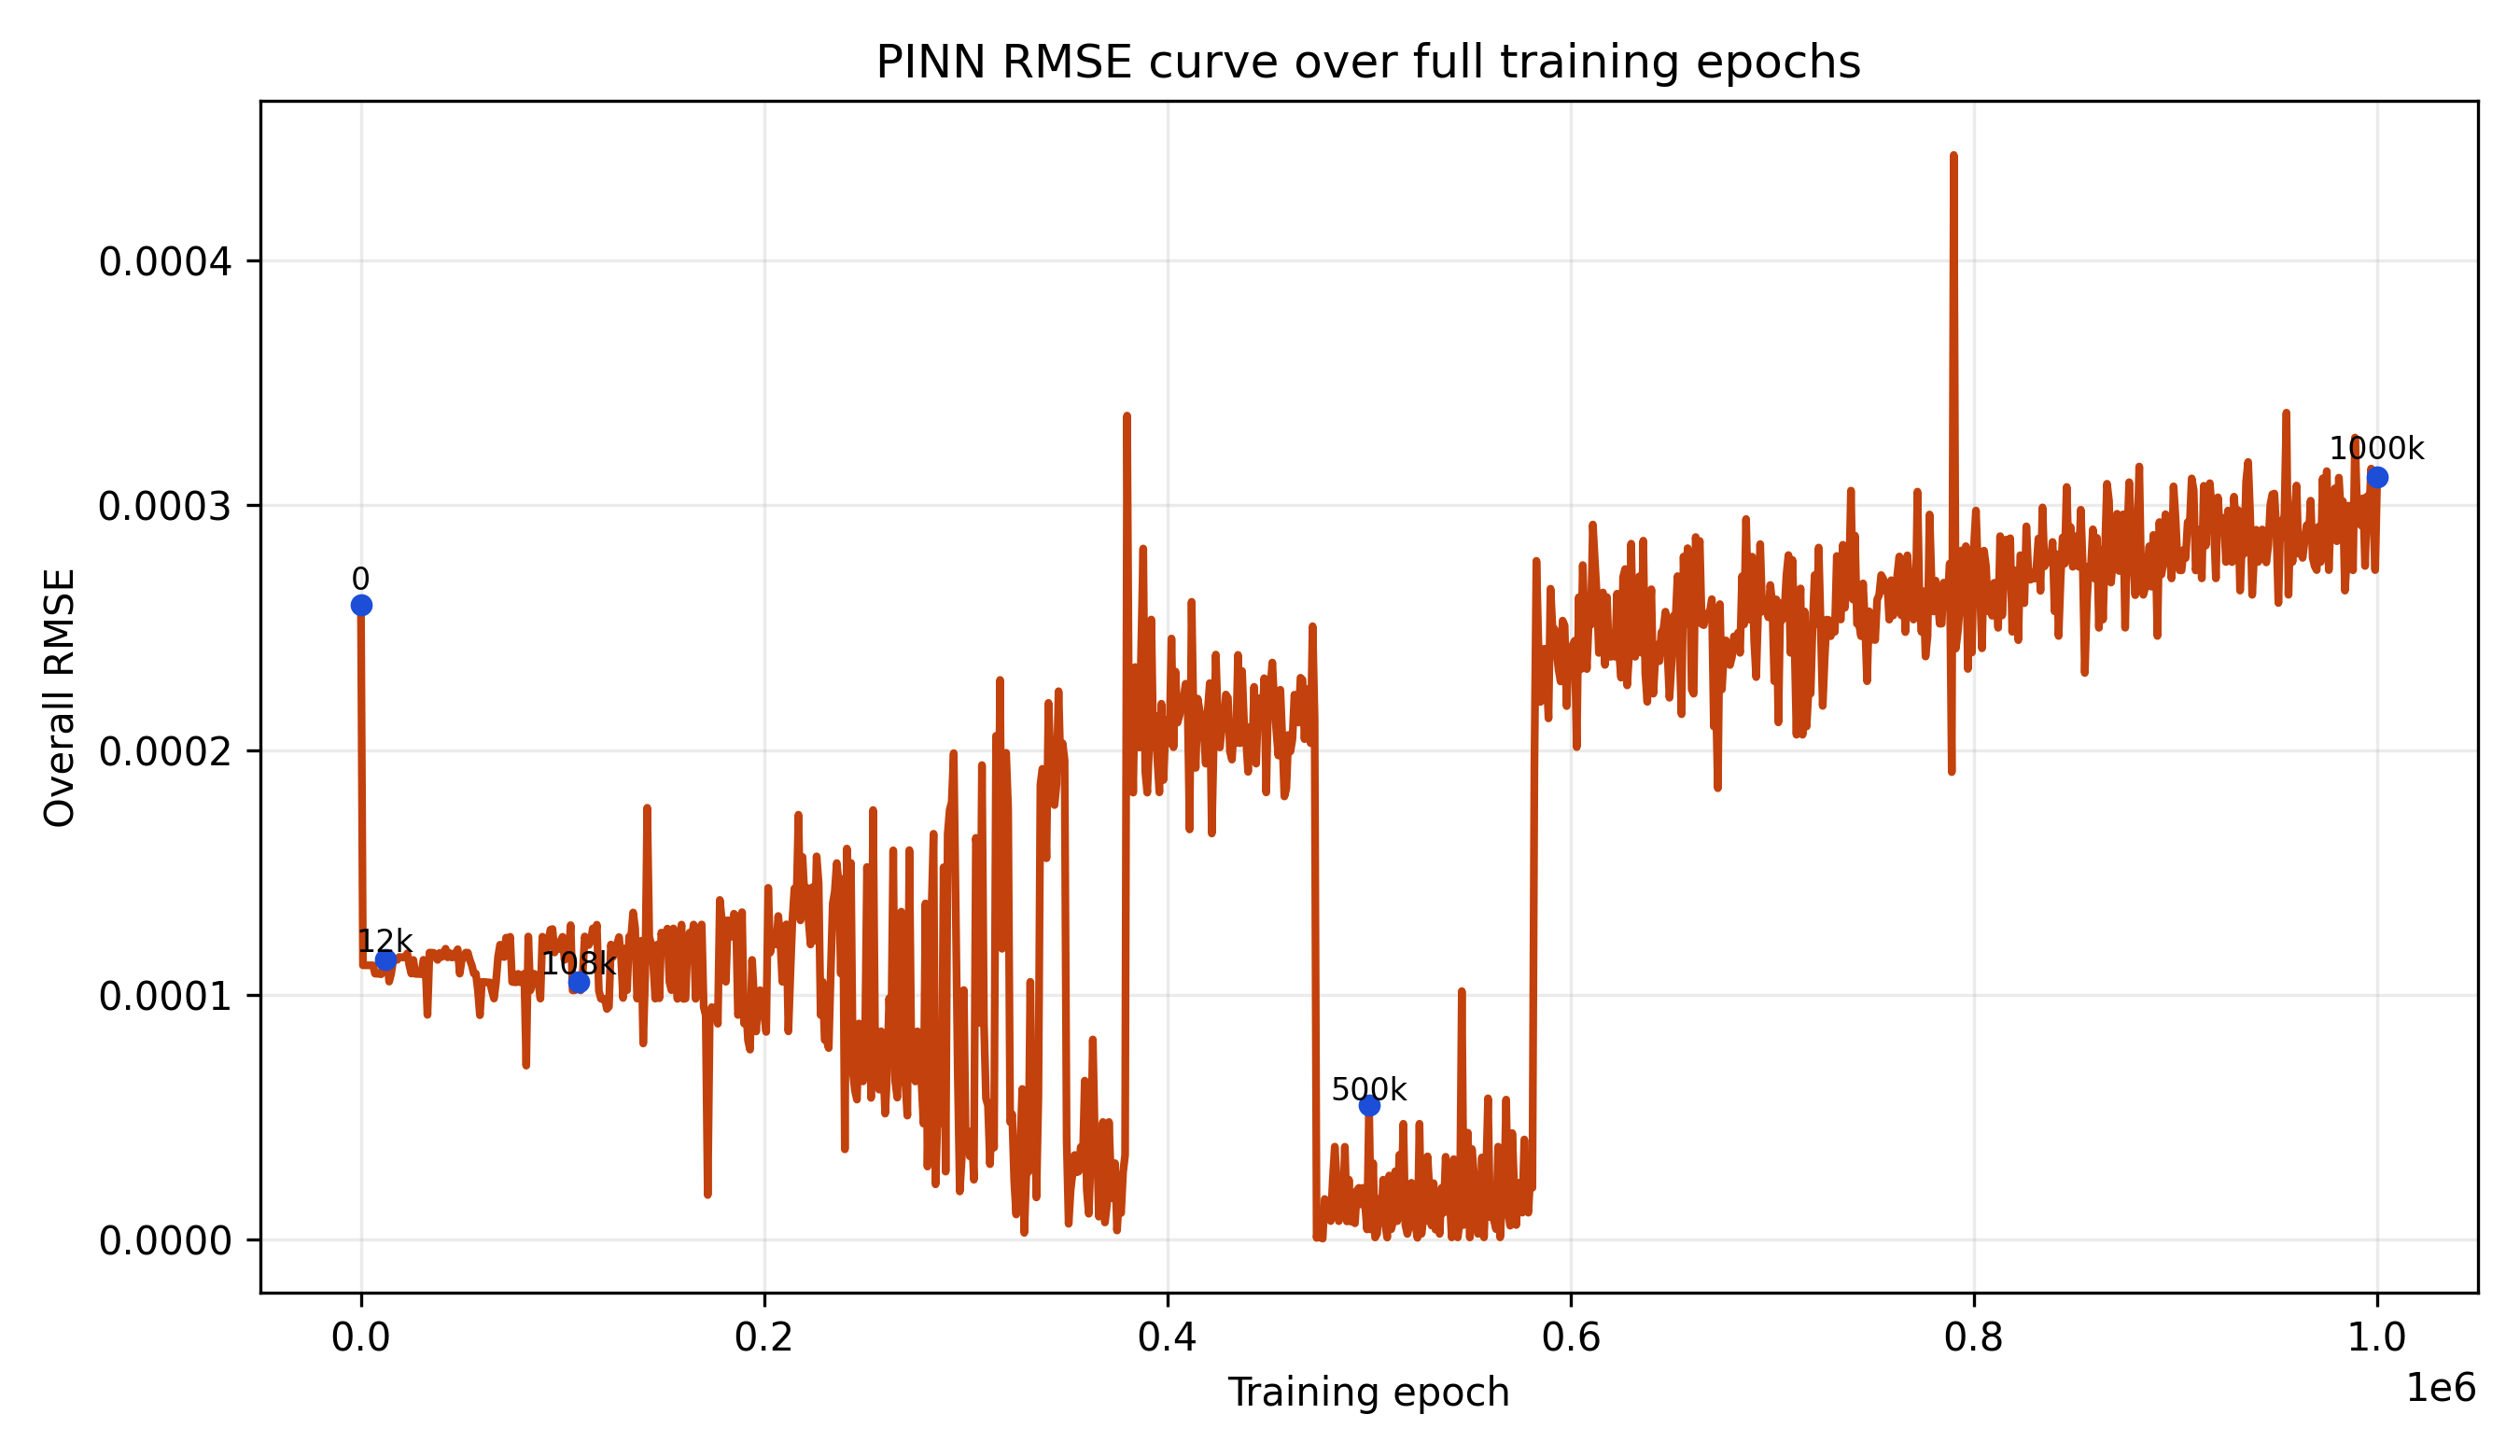
\includegraphics[width=0.82\textwidth]{fig5_5_pinn_full_epoch_rmse.png}
  \caption{PINN 全训练轮次 RMSE 变化曲线}
  \label{fig:pinnfullrmse}
\end{figure}

\subsection{FNO 结果分析}

根据 \texttt{web\_exports/fno/epoch\_108000/metrics.json}，FNO 在 \texttt{epoch\_108000} 时的整体 MSE 为 $1.194\times10^{-7}$，整体 RMSE 为 $3.456\times10^{-4}$。同时，FNO 在 \texttt{epoch\_012000} 和 \texttt{epoch\_060000} 时的 RMSE 分别为 $1.329\times10^{-3}$ 和 $3.926\times10^{-4}$，说明其误差会随着训练轮次增加而持续下降，但在当前任务中最终精度仍低于 PINN。

\begin{figure}[H]
  \centering
  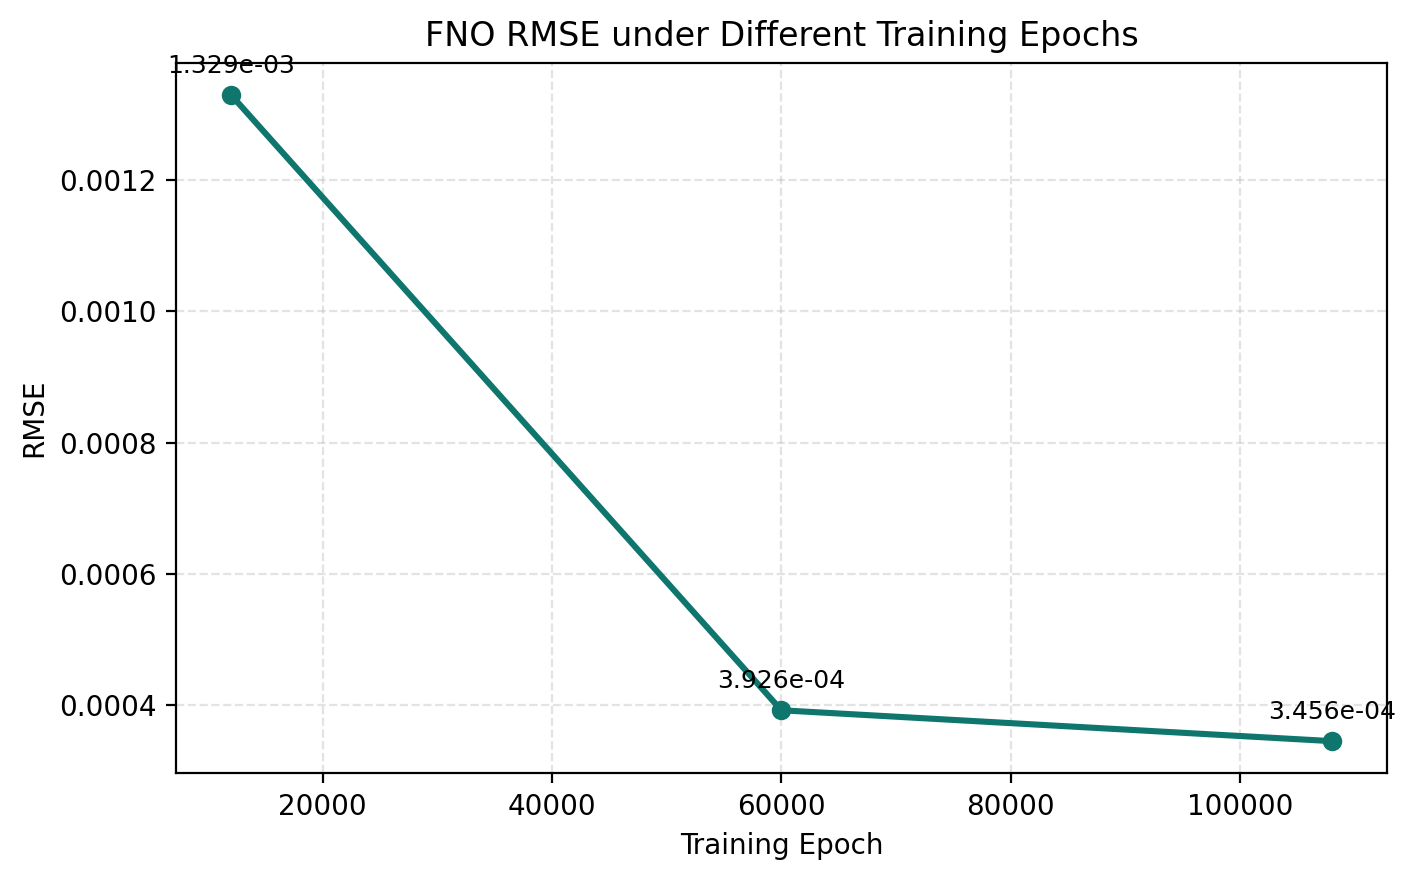
\includegraphics[width=0.72\textwidth]{fig5_4_fno_epoch_rmse.png}
  \caption{FNO 不同训练轮次 RMSE 变化曲线}
\end{figure}

\subsection{PINN 与 FNO 对比分析}

在相同方程、相同网格与统一真值条件下，PINN 与 FNO 的核心指标如表 \ref{tab:modelcmp} 所示。需要说明的是，本文比较的目标并不是宣称两类模型在理论上完全等价，而是在统一应用任务下对两类模型的结果表现进行工程性与实验性比较。为保证比较尽可能公平，本文遵循以下原则：其一，PINN 与 FNO 都针对同一二维热方程任务进行结果导出；其二，两者均在 $101\times101$ 网格下与同一解析真值进行比较；其三，比较所使用的短时/长时回放窗口和前端展示链路保持一致；其四，整体 MSE、整体 RMSE、逐帧 MSE 和逐帧 RMSE 采用同一套计算方式。因此，本文结论应理解为“在当前统一实验任务与统一评价标准下，PINN 与 FNO 的结果对比”，而不是对两类方法全部应用场景的绝对优劣判断。
\begin{table}[H]
  \centering
  \caption{PINN 与 FNO 结果对比}
  \label{tab:modelcmp}
  \begin{tabular}{llll}
    \toprule
    模型 & 结果集 & 整体 MSE & 整体 RMSE \\
    \midrule
    PINN & epoch\_108000 & $1.039\times10^{-8}$ & $1.020\times10^{-4}$ \\
    FNO & epoch\_108000 & $1.194\times10^{-7}$ & $3.456\times10^{-4}$ \\
    \bottomrule
  \end{tabular}
\end{table}

两者 RMSE 比值约为
\begin{equation}
\frac{\mathrm{RMSE}_{\mathrm{FNO}}}{\mathrm{RMSE}_{\mathrm{PINN}}}\approx 3.39.
\end{equation}
这表明在当前二维热方程任务上，PINN 的最终精度优于 FNO。与此同时，平台的对比热力图与差异图也说明两类模型在整体扩散趋势上保持一致，但在局部区域仍存在可观察的空间偏差。

\begin{figure}[H]
  \centering
  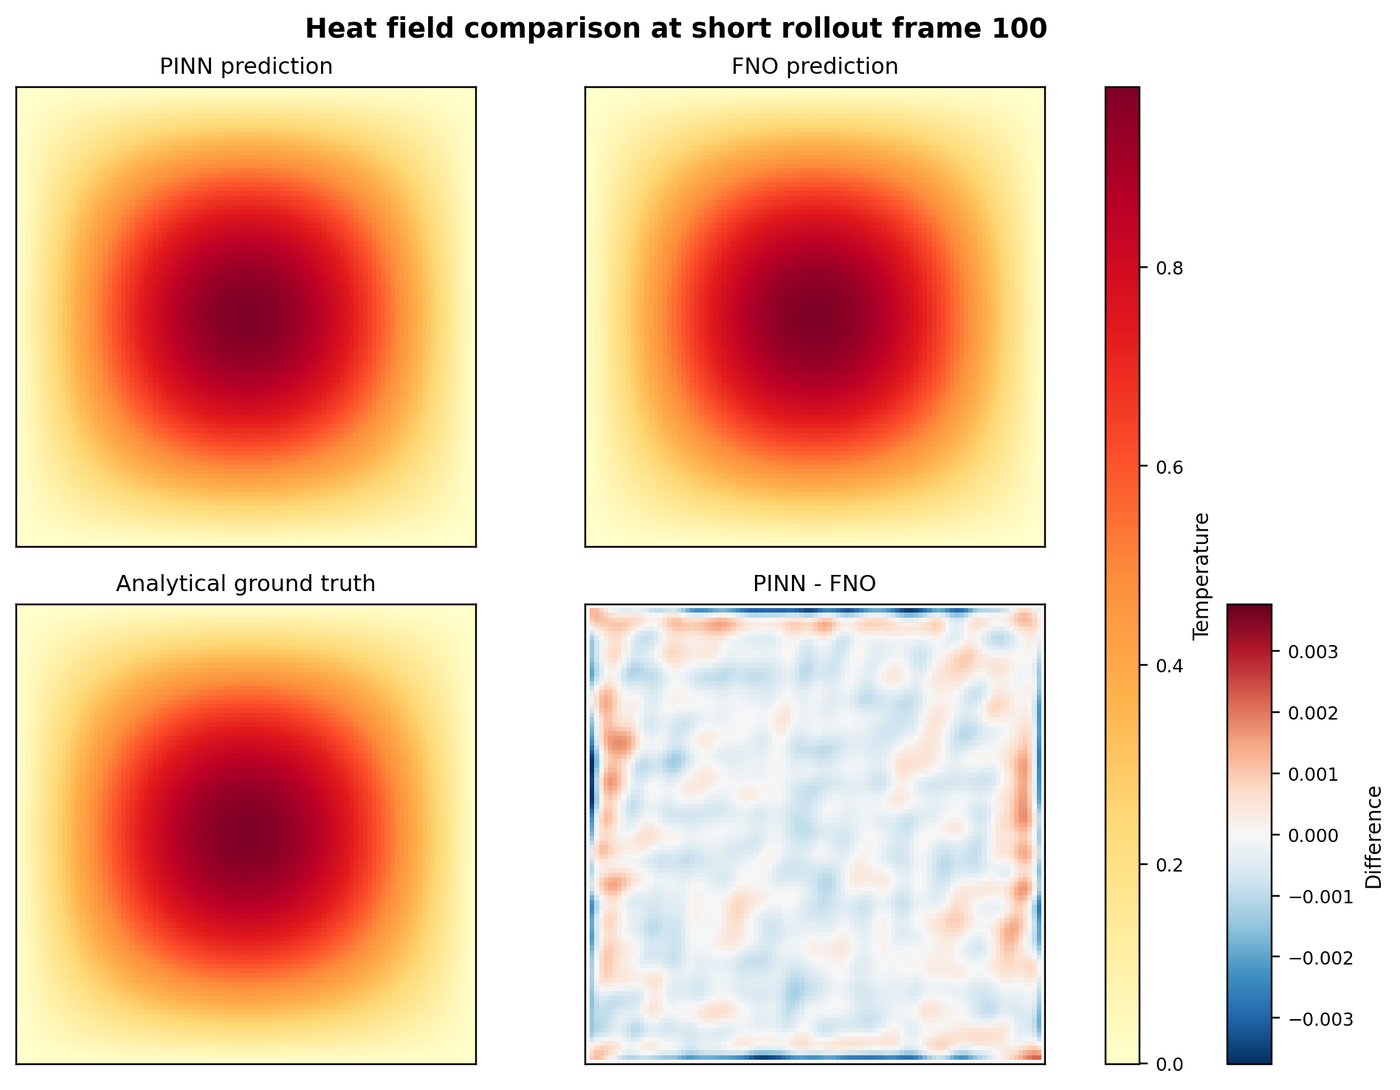
\includegraphics[width=0.88\textwidth]{fig5_1_heatmap_comparison.png}
  \caption{PINN、FNO 与解析真值热力图对比}
\end{figure}

\begin{figure}[H]
  \centering
  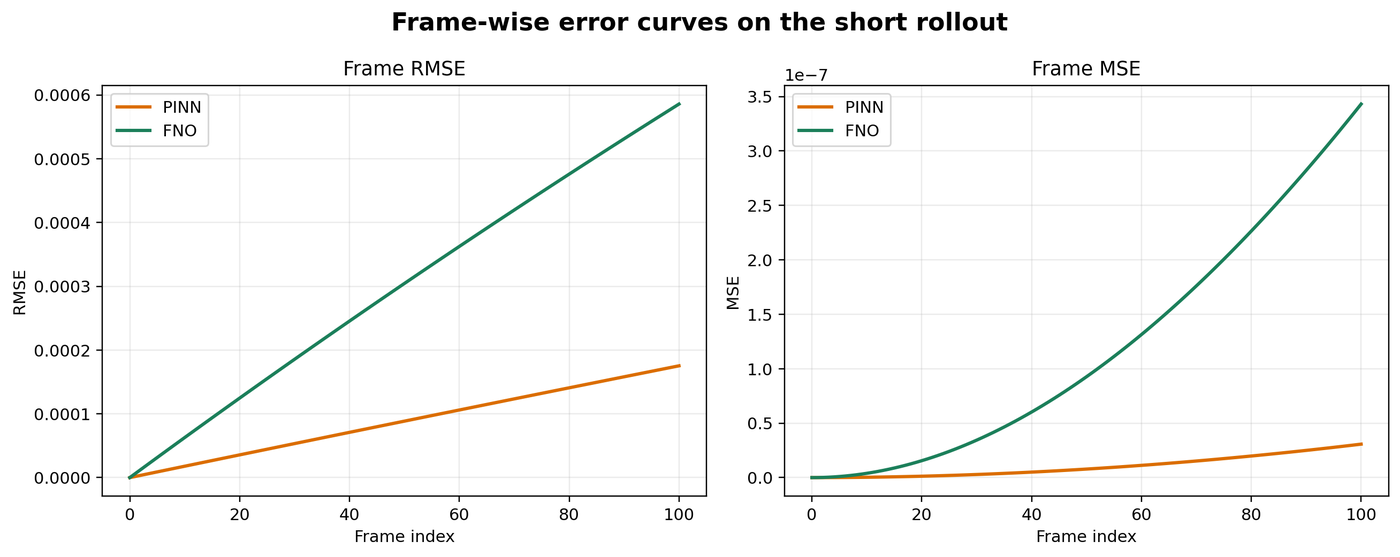
\includegraphics[width=0.88\textwidth]{fig5_2_error_curves.png}
  \caption{PINN 与 FNO 的逐帧误差曲线对比}
\end{figure}

\subsection{平台展示与系统测试分析}

平台测试主要从结果读取、参数映射和可视化联动三个角度展开。结果表明：
\begin{enumerate}[label=\arabic*)]
  \item PINN 与 FNO 结果目录能够被统一识别并正常读取；
  \item 参数化演示区能够根据输入参数稳定匹配至对应的 PINN 预计算结果；
  \item 对比分析区能够同步展示 PINN、FNO、Ground Truth 和差异热力图，并联动误差曲线。
\end{enumerate}

结合当前页面布局，平台测试与展示结果可进一步概括为三点。其一，PINN 参数化演示区能够在不触发新训练任务的前提下，直接根据参数组回放对应热图结果，从而降低演示等待时间。其二，PINN/FNO 对比区在同一页面下集成了 PINN 热图、FNO 热图、解析真值、差异图以及 Frame RMSE/Frame MSE 曲线，使“局部空间差异”和“整体误差趋势”可以同步观察。其三，状态芯片、结果集标识和参数映射摘要共同构成了页面的信息导航层，使前端不仅能“展示图”，也能清楚说明“当前展示的是什么结果、结果来自哪一组参数、比较使用的是哪一组运行结果”。

\subsection{补充讨论：参数回放、训练轮次展示与后续扩展}

当前平台的参数化模块本质上是“参数回放系统”，而不是“在线训练系统”。这种设计的主要原因在于原始 PINN 训练过程耗时较长，现场重新训练不适合答辩展示。通过提前导出正式结果并建立参数映射机制，平台能够在保证稳定性的同时保留交互感。

此外，随着原始 PINN 训练过程导出更多 \texttt{epoch\_xxxxxx} 结果，平台还可扩展为“训练轮次可视化”模式，即通过训练轮次滑块观察同一热方程任务下热图如何随训练过程逐步收敛。该部分属于平台的自然扩展方向，可在现有统一结果结构之上直接实现，无需重新设计数据接口。

\section{总结与展望}

本文围绕“流体模拟自动化平台”完成了系统设计、结果组织与实验分析工作。平台当前以二维热方程为真实验证对象，保留原始 PINN 模块的核心算法结构，实现了非侵入式接入；同时将 FNO 结果作为离线对照模型接入统一展示链路。这里“自动化”主要体现在结果读取、参数匹配、播放展示和模型对比四个方面。前端页面将 PINN 参数化演示与 PINN/FNO 对比分析拆分为两大部分，形成了兼顾工程展示与论文分析的完整结构。

实验结果表明，在当前热方程任务中，PINN 的整体精度优于 FNO，且误差传播更为平缓。平台采用“参数填写后匹配预计算结果”的展示机制，保证了系统展示稳定性，也使论文的系统部分与实验部分之间形成了清晰分工：前者强调统一结果标准与可视化平台，后者强调 PINN 与 FNO 的对比研究。

后续工作可从以下几个方向展开：一是继续补充更多离线 PINN 结果集，以支持更细粒度的训练轮次展示与参数敏感性分析；二是扩展更多偏微分方程任务，如 Poisson 方程、Burgers 方程以及更一般的流体方程，使当前热方程验证案例逐步过渡到更完整的流体模拟任务；三是进一步完善前端图表和界面布局，使平台更适合教学展示与答辩演示。

\clearpage
\phantomsection
\addcontentsline{toc}{nonumbersection}{参考文献}
\bibliographystyle{gbt7714-numerical}
\bibliography{refs}

\clearpage
\addcontentsline{toc}{nonumbersection}{致谢}
\begin{center}
    \zihao{3} \textbf{致谢} \\
\end{center}

在本次毕业设计与论文撰写过程中，指导教师甘言海老师在选题定位、系统设计和论文修改等方面给予了耐心指导与帮助。在此表示诚挚感谢。同时，也感谢相关课程教师和同学在项目实现、文献检索和界面演示等环节中提供的支持。最后，感谢家人对本人学习和毕业设计工作的理解与鼓励。

\end{document}
